\chapter{Photometry of NGC\,6791 \& NGC\,6819 Red Giant Cluster Members}
\label{chap:red_giants}

% \section*{abstract}
%     In this chapter we present global asteroseismic parameters for all red giant (RG) cluster members of NGC\,6791 and NGC\,6819. We selected these RGs based on our membership determinations from the previous chapter. We corrected the instrumental perturbations present in the raw light curves for all red giant cluster member candidates and selected the light curve corrections resulting in the highest red giant excess signal-to-noise. We present a complete database of the extracted global asteroseismic parameters of $\nu_\mathrm{max}$, $\Delta\nu$, $\epsilon$, and the stellar granulation parameters, and compare the cluster ensembles to the full \Kepler{} targeted ensemble.
\newpage

\section{Introduction to Solar-like oscillators}

\cite{leighton_velocity_1962} first observed the five minute oscillations in the Sun. These are now known to be stochastically driven and intrinsically damped by turbulent motion in the convective envelope. Solar-like oscillators refers to all variable stars with oscillation modes excited through this process of stochastic turbulence in the convective envelope. Therefore, these oscillations should be present in any star with a significant convective envelope, including low-mass (M $\leq 1.6$\,\Msol{}) main sequence stars, subgiant stars and red giant stars \citep{aerts_current_2008}. 

Solar-like oscillation modes typically exhibit p-mode behaviour in the convective envelope, where they are predominantly acoustic in character with a pressure-driven restoring force. Theory also predicts g-mode behaviour in the core, where buoyancy is the restoring force. Figure \ref{fig:modes} shows ray paths for p-modes (left) and g-modes (right) within a solar-like star. The p-modes penetrate deeper into the stellar interior when they are of lower angular degree, whilst g-modes are typically restricted to the radiative core, being evanescent in stellar convective zones.

As discussed in \cref{chap:intro:astero}, we can detect these oscillations by taking precise measurements of photometric changes. There have been a number of space-based missions over the past two decades including \textsc{Most} \citep{rucinski_most_2003}, \textsc{CoRoT} \citep{michel_corot_1998}, \Kepler{} and \textit{K2} \citep{borucki_kepler_2009}, and now \textsc{Tess} \citep{ricker_transiting_2014}, that have provided high-precision photometric data for thousands of solar-like stars. This data has led to a revolution in our understanding of their stellar structure and processes. Many large surveys of solar-like oscillators have been conducted \cite[eg.][]{stello_detection_2010,hekker_characterization_2011,mosser_characterization_2012,mosser_mixed_2014,yu_asteroseismology_2018-1} with \cite{hon_search_2019} having conducted the largest and most comprehensive search for evolved solar-like oscillators, detecting oscillations in $\sim22\,000$ red giant stars in long cadence light curves of the $\sim197\,000$ targeted stars in the \Kepler{} nominal field of view.

The study of solar-like oscillations has wide-reaching applications for stellar astrophysical studies including: determining stellar ages \citep{silva_aguirre_ages_2015, bellinger_seismic_2020}, probing core rotation \citep{beck_kepler_2011, mosser_probing_2012, deheuvels_seismic_2014}, studying the possibility of stellar core magnetic fields \citep{fuller_asteroseismology_2015, stello_suppression_2016, stello_prevalence_2016, loi_torsional_2017, loi_low-degree_2020}, ensemble analyses of intrinsic stellar properties such as radius and mass \cite[eg.][]{garcia_asteroseismology_2018, hekker_giant_2017}, ensemble analyses of mass loss in later evolutionary stages \citep{miglio_asteroseismology_2012}, and informing Galactic evolutionary studies \citep{casagrande_photometric_2015, sharma_stellar_2016, silva_aguirre_confirming_2018}.

The analysis of solar-like oscillators in open clusters is particularly important, as an ensemble analysis can leverage the similar stellar ages and metallicities of cluster members to constrain free parameters in comparative stellar models. This allows for seismic membership determinations \citep{stello_detection_2010,stello_asteroseismic_2011,bellamy_using_2015}, studies of stellar rotation and thus inclination angle from dipole mode splitting \citep{corsaro_spin_2017}, and mass loss in red giant evolutionary stages \citep{miglio_asteroseismology_2012}. For a review of the current state of asteroseismology of solar-like oscillators we direct the reader to \cite{chaplin_asteroseismology_2013}.

Stellar oscillations are typically analysed by taking the Fourier transform of the light curves. For modes to be detected in regularly-sampled data, the observations must be sampled with a cadence ($\delta t$) such that the acoustic cutoff frequency is below the Nyquist frequency of the observations:

\begin{equation}
    \nu_{\mathrm{Nyq}} = \cfrac{1}{2\,\delta t} .
    \label{eqtn:nyq}
\end{equation}

Figure \ref{fig:rgps} shows a typical log-scaled power spectrum of a red giant solar-like oscillator. This spectrum consists of three characteristic features: (a) At low frequencies turbulent surface convection typically dominates, resulting in the frequency dependent granulation background, (b) The p-mode envelope, also called the power excess, is evident around $56\,\mu$Hz in the form of a sequence of relatively narrow peaks following a regularly spaced pattern on top of the background signal, and (c) Close to the Nyquist frequency the power spectrum tends to a flat profile where the photon noise (white noise) dominates. In addition, stellar activity features such as spots and flares, convolved with the geometry of the observer's view, can introduce peaks and harmonics to the granulation background at low frequencies.

\begin{figure}
    \centering
    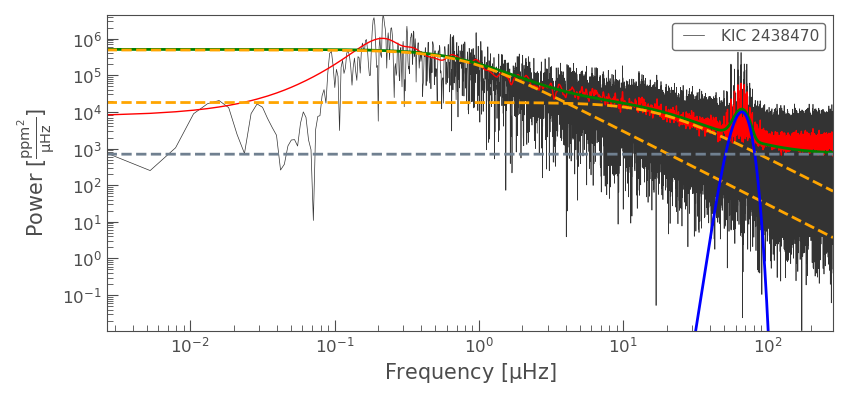
\includegraphics[width=0.99\linewidth]{Chapter5/2438470_ps_harvey.png}
    \caption[Power spectrum of a typical Red Giant solar-like oscillator]{Power spectrum of KIC 2438470, a typical Red Giant solar-like oscillator. A Gaussian-smoothed power spectrum using a $0.1\,\mu$Hz window (red line) is overlaid. The two Harvey components characterising the granulation background (orange dashed lines), a Gaussian fit to the p-mode power excess (blue line) and a constant white noise (grey dotted line) component are overlaid. The total power of the fitted model is also shown (green line).}
    \label{fig:rgps}
\end{figure}

The background convective signal can be effectively described by a Harvey function \citep{harvey_high-resolution_1985}:

\begin{equation}
    P(\nu) = \eta_\mathrm{a}(\nu)^2 \sum_{i} \cfrac{4\sigma_i^2\tau_i}{1+(2\pi\nu\tau_i)^2} + P'_n
    \label{eqtn:Harvey}
\end{equation}

where 

\begin{equation}
    \eta_\mathrm{a}(\nu)^2 = \sinc^2{\left[\cfrac{\pi}{2}\left(\cfrac{\nu}{\nu_{\mathrm{Nyq}}}\right)\right]}
    \label{eqtn:apod}
\end{equation}

\noindent is the apodization factor arising from finite observations, $\sigma_i$ and $\tau_i$ are the amplitude and characteristic timescale of the $i$-th Harvey component \citep{mathur_granulation_2011}, and $P'_n$ is the white noise level. \cite{karoff_observations_2013} and \cite{kallinger_connection_2014} have shown that two Harvey components are sufficient in most cases to describe this background.

The p-mode envelope can be approximately described by a Gaussian \citep{kallinger_evolutionary_2012} and measurements of the modes allows for the extraction of average ``global'' seismic parameters, including:

\begin{itemize}
    \item $\nu_{\mathrm{max}}$ - The frequency at maximum power \citep{kjeldsen_amplitudes_1995, brown_detection_1991}
    \item $\Delta\nu$ - The large frequency separation between radial modes of consecutive order.
    \item $\delta\nu_{nl}$ - The small frequency separations
    \item $\epsilon$ - A phase term dependent on near-surface region properties
\end{itemize}

The frequency at maximum power, $\nu_{\mathrm{max}}$, is linked empirically to the acoustic cutoff frequency, and combined with measurements of the effective temperature, $T_{\mathrm{eff}}$ (eg. from spectroscopy), allows for the direct measurement of surface gravity, $g$, and thus stellar mass and radius:

\begin{equation}
    \nu_{\mathrm{max}} = \cfrac{g}{\sqrt{T_{\mathrm{eff}}}} \;\; \propto \; \cfrac{M}{R^2 \sqrt{T_{\mathrm{Teff}}}}.
\end{equation}

The individual modes that comprise the power excess are regularly spaced in a pattern that is predicted by asymptotic theory \citep{tassoul_asymptotic_1980, gough_solar_1986} with frequencies approximated by:

\begin{equation}
    \nu_{nl} \simeq \left(n +\cfrac{l}{2} + \epsilon \right)\Delta\nu - \delta\nu_{0l},
    \label{eqtn:modes}
\end{equation}
% \begin{equation}
%     \nu_{nl} \simeq \left(n +\cfrac{l}{2} + \epsilon \right)\Delta\nu - \left[Al(l+1)-\delta\right]\cfrac{\Delta\nu^2}{\nu_{nl}}
% \end{equation}

\noindent where $n$ and $l$ are the radial order and angular degree of the specific modes, and $\delta\nu_{0l}$ is a small correction factor that is zero for $l = 0$ modes. The large frequency separation, $\Delta\nu$, is proportional to the sound travel speed across the star and is a direct measure of the mean stellar density \citep{ulrich_determination_1986}.

The phase term, $\epsilon$, is related to the near-surface structure where p-modes are reflected, and is a dimensionless offset of the radial modes typically with a value between 0.5 and 1.5. \cite{christensen-dalsgaard_asymptotic_2014} showed the different locations of the second helium ionisation zone within red clump and red giant branch stars results in different values of $\epsilon$, enabling its use in stellar evolutionary state determinations.

The small frequency separations, $\delta\nu_{02}$ and $\delta\nu_{13}$, depend on the composition of the stellar interior. In main-sequence stars, the low-angular-degree modes probe the core helium content and so are indicators for stellar age \citep{christensen-dalsgaard_introductory_1984, ulrich_determination_1986, christensen-dalsgaard_overview_1988}. In subgiant and red giant stars the turning points of these modes occur before they reach the core. Therefore, in these stars the small frequency separations scale with the large frequency separation instead of probing the evolutionary stage.

The small frequency separation $\delta\nu_{01}$ describes the offset of the dipole modes from the midpoint of the $l = 0$ modes. In main sequence stars, this value probes the stellar core conditions. In red giants, the turning point for the dipole modes occurs at the base of the convective envelope, allowing this small frequency separation to be used as an evolutionary state diagnostic. Typically, red giant branch stars have small, negative values for this separation, whilst in the more evolved red clump stars this offset is positive \citep{montalban_seismic_2010}.

In main-sequence stars, oscillations are purely p-mode in behaviour as g-modes are evanescent in convective regions. For red giants however, all non-radial modes have mixed character with g-mode behaviour in the core and p-mode behaviour in the envelope. This is due to p- and g-modes coupling, resulting in deviations from the regular frequencies of uncoupled modes described by Equation \ref{eqtn:modes} from avoided crossings.

\subsection*{\'Echelle Diagrams}
\label{sect:ech}
\'Echelle diagrams \citep{grec_full-disk_1983} provide a useful diagnostic for displaying and extracting some of these global parameters. Figure \ref{fig:echelle} shows a typical \'echelle diagram for KIC 2438470, constructed by dividing the power spectrum into equal segments of width $\Delta\nu = 6.44\,\mu Hz$, that are then stacked vertically. The $l = 0$ (red circles) and $l = 2$ modes (blue triangles) form roughly vertical ridges, while $l = 1$ modes (black squares) typically show deviations resulting from mixed mode characteristics. All modes are also affected by large-scale stellar structural features that result in curvature of the ridges. To measure the phase shift, $\epsilon$, from an \'echelle diagram, we measure the fractional distance to the $l = 0$ ridge. \cite{huber_asteroseismology_2010} and \cite{white_asteroseismic_2011} have shown $\epsilon$ typically has a value between 0.5 and 1.5, so it may be necessary to add 1 to the resulting fractional distance to get the correct phase shift. The global small frequency separations can also be extracted using this diagram by fitting vertical lines to the centre of the mode ridges and measuring the relevant distances.

\begin{figure}
    \centering
    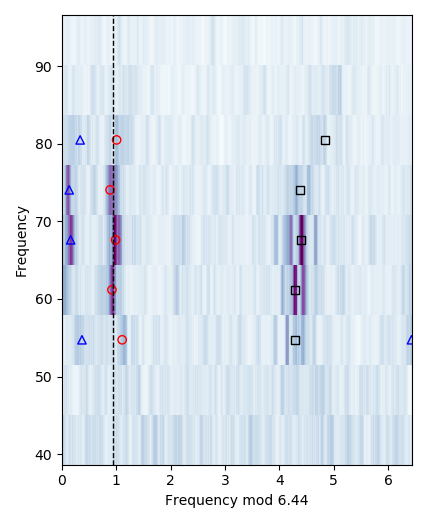
\includegraphics[height=0.5\textheight]{Chapter5/echelle_2438470_somemodes.png}
    \caption[Typical \'echelle diagram for a Red Giant solar-like oscillator]{\`Echelle diagram for KIC\,2438470 with a large frequency separation of $6.44\,\mu\mathrm{Hz}$. The approximate positions of the $l = 0$ modes (red circles), $l = 1$ modes (black squares) and $l = 2$ modes (blue triangles) are plotted. The offset of the $l=0$ ridge due to the phase term, $\epsilon$, at a modulus of 0.929 ($\epsilon = 1.144$) is also highlighted (dashed line). }
    \label{fig:echelle}
\end{figure}

\subsection*{Scaling Relations}

\cite{brown_detection_1991} and \cite{kjeldsen_amplitudes_1995} proposed scaling relations to estimate the global seismic parameters of \numax{} and \dnu{} in solar analogs based on intrinsic stellar properties:

\begin{equation}
    \cfrac{\nu_{\mathrm{max}}}{\nu_{\mathrm{max},\odot}} \simeq \cfrac{M/M_{\odot}\left(T_{\mathrm{eff}}/T_{\mathrm{eff},\odot}\right)^{3.5}}{(L/L_{\odot})}
    \label{eqtn:numax_scaling}
\end{equation}

\begin{equation}
    \cfrac{\Delta\nu}{\Delta\nu_{\odot}} \simeq \cfrac{\left(M/M_{\odot}\right)^{0.5}\left(T_{\mathrm{eff}}/T_{\mathrm{eff},\odot}\right)^{3}}{(L/L_{\odot})^{0.75}} .
    \label{eqtn:deltanu_scaling}
\end{equation}

% \begin{equation}
%     \cfrac{\nu_{\mathrm{max}}}{\nu_{\mathrm{max},\odot}} = \cfrac{M/M_{\odot}}{(R/R_{\odot})^2\sqrt{T_{\mathrm{eff}}/T_{\mathrm{eff},\odot}}}
%     \label{eqtn:numax_scaling}
% \end{equation}

% \begin{equation}
%     \cfrac{\Delta\nu}{\Delta\nu_{\odot}} = \cfrac{(M/M_{\odot})^{1/2}}{(R/R_{\odot})^{-3/2}} 
%     \label{eqtn:deltanu_scaling}
% \end{equation}

\noindent These equations can be rearranged to give the seismic scaling relations:

\begin{equation}
    \cfrac{M}{M_{\odot}} \simeq \left(\cfrac{\nu_{\mathrm{max}}}{\nu_{\mathrm{max},\odot}}\right)^3 \left(\cfrac{\Delta\nu}{\Delta\nu_{\odot}}\right)^{-4}\left(\cfrac{T_{\mathrm{eff}}}{T_{\mathrm{eff},\odot}}\right)^{3/2} ,
    \label{eqtn:mass_scaling}
\end{equation}

\noindent and

\begin{equation}
    \cfrac{R}{R_{\odot}} \simeq \left(\cfrac{\nu_{\mathrm{max}}}{\nu_{\mathrm{max},\odot}}\right)\left(\cfrac{\Delta\nu}{\Delta\nu_{\odot}}\right)^{-2}\left(\cfrac{T_{\mathrm{eff}}}{T_{\mathrm{eff},\odot}}\right)^{1/2} ,
    \label{eqtn:radius_scaling}
\end{equation}


\noindent first used by \cite{stello_oscillating_2008} and \cite{kallinger_asteroseismology_2010} to estimate intrinsic stellar parameters from asteroseismic observations. The value of $\Delta\nu$ in these relations is not directly determined from individual oscillation modes, but rather refers to the gradient of the best-fit linear trend between the radial order (n) and the oscillation frequencies ($\nu_{nl}$). In red giants, the presence of mixed modes beyond the $l = 0$ angular degree restrict this calculation to the radial modes. We note that these scaling relations rely on the assumption the frequencies closely follow the asymptotic relation, which is only true when $n >> l$ and when the stars investigated are essentially homologous to the Sun. In the case of the red giants investigated here these assumptions do not strictly hold true \citep{mosser_asymptotic_2013, belkacem_seismic_2013}, however, some of the deviations introduced as a result of these assumptions effectively cancel out \citep{white_asteroseismology_2013}, and the overall intrinsic stellar properties work out fairly well.

These scaling relations have been extensively applied to the ensemble of asteroseismic observations available from the \textsc{CoRoT}, \Kepler{}, and K2 missions, with many investigations focusing on the accuracy of the estimated intrinsic stellar properties and suggesting small corrections \cite[e.g.][]{basu_determination_2010, white_calculating_2011, miglio_asteroseismology_2012}. For a more detailed summary of these corrections we refer the reader to \cite{hekker_scaling_2020}. 


%
%SCALING RELATIONS!!!!

% The photometric variations in these stars are dominated by surface granulation and the oscillation modes, both of which depend on the surface gravity of the star. 

% Solar-like oscillators
% - global params, echelle diagrams
% Seismic membership (Stello '10, '11)
% Previous red giant results including params, rotation, angle of inclination etc


\section{Cluster light curve processing}
\label{sect:lc_select}

Isabel Colman has produced raw light curves for all cluster members in the 200\,px $\times$ 200\,px \Kepler{} superstamp images of the cluster centres of NGC\,6791 and NGC\,6819 \citep{colman_pixels_2020}. The quality metadata for the superstamp images is generalised to the entire image, providing no localised quality information for a given target. As such, \cite{colman_pixels_2020} made no photometric cuts based on this metadata, and provided no quality flag field for the extracted light curves. The rest of this chapter describes my analysis of these light curves, which were extracted by Isabel using a custom image subtraction code to target stars that I identified in \cref{chap:membership} as likely members (meanprob $\ge 0.03$). Isabel made an additional cut, restricting the standard deviation of the membership score distribution, stdprob, to be stdprob $\leq 0.3$. This cut was made to minimize the chance of extracting foreground and background non-members whose motion and position were not well constrained or coincidentally fell near the edge of the distribution of cluster values. To select the likely red giant members, I made photometric cuts of $G \leq 17.25$ and $G_{BP}-G_{RP}\ge1.25$.

The image subtraction code limits the extraction of data to stars that are at least 2\,pixels from the superstamp edge in a given quarter. As such, stars located close to the image edges may have missing quarters of data in the image-subtracted light curves due to small shifts in the telescope pointing between quarters. These missing quarters tend to fall on the same CCD and result in a regular window function that results in individual oscillation modes being split into clusters of aliased frequencies centred around the actual oscillation frequency. We compared the available image-subtracted data to the \Kepler{} targeted data, and in those cases where additional quarters of data are available, appended the simple aperture photometry (SAP) from the targeted quarters to our image-subtracted light curve. To maintain consistency in terms of quality flags, all data from the SAP light curves was included.

\Kepler{} light curves show a number of instrumental perturbations that must be corrected prior to searching for solar-like oscillations. This is especially important for detecting low-amplitude oscillations. Within single-quarter observations, these perturbations include outliers, discontinuous jumps in the mean observed flux, short-term low-frequency drifts associated early in the mission with instrument temperature changes after safe-mode events \citep{garcia_preparation_2011}, and later with thermal changes during monthly data downlinks, and CCD-specific, quarter-long, low-frequency trends. From quarter to quarter there are also discontinuous jumps and CCD sensitivity changes resulting from the rotation of the \Kepler{} spacecraft. Figure \ref{fig:lc_system} shows examples of these instrumental perturbations. 

\begin{figure}
    \centering
    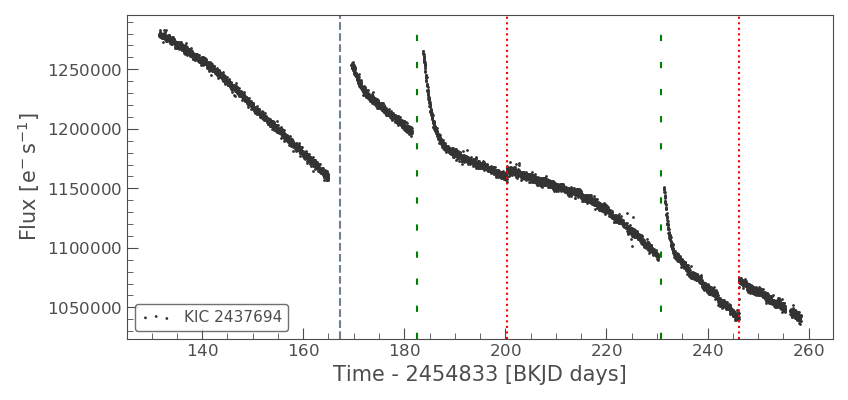
\includegraphics[width=\linewidth]{Chapter5/lc12_systematics.png}
    \caption[Light curve of KIC 2437694 showing quarters 1 and 2]{Light curve of KIC\,2437694 showing quarters 1 and 2. The quarter to quarter CCD sensitivity jump (grey dashes), thermal drifts (green dashes), and discontinuous jumps (red dashes) are shown. Long-term low-frequency trends specific to the CCD can also be seen as general slopes or low-order polynomial trends inherent in each quarter.}
    \label{fig:lc_system}
\end{figure}

Whilst the exoplanet community have developed a number of de-trending algorithms to correct \Kepler{} systematics, these tools have been designed to search for transits that are typically small-amplitude periodic signals are localised in time. In contrast, stellar oscillations are present throughout the entire time series of the light curve in essentially stable modes. In particular, the thermal ramping effects and consequent changes in statistical noise characteristics in the first 2-3\,days of data following downlinks are challenging to overcome for exoplanet searches and are typically removed. However, introducing larger gaps in the time series (beyond the downlink gap), results in an increased window function within the Fourier transform typically used to analyse asteroseismic signals. This decreases the sensitivity of searches for solar-like oscillations, particularly for those in the higher-frequency and lower-power regime (less evolved solar-like oscillators). For asteroseismic analyses, large discontinuous changes in flux must be corrected for as they generate power at many frequencies, but changes in noise properties from one segment to another are less of an issue, provided they are not too severe.

\subsection{Correction Methods}

We investigated three different correction processes to remove instrumental perturbations within each quarter: high-pass filtering using a custom Gaussian filter, polynomial de-trending, and Co-trending Basis Vectors (CBVs). We initially corrected all of our extracted light curves with a simple Gaussian high-pass filter designed to account for the irregularly sampled data with missing data points. We applied this filter on a quarter by quarter basis to each light curve with window widths equivalent to 0.5\,d, 1\,d, and 2\,d standard deviation Gaussians. This process is sufficient for stars with high frequency variations but removes all low-frequency trends, including the oscillation power excesses of red giants with \numax{} lower than about 15\,$\micro$Hz. It also affects the extraction of the granulation signal parameters for these stars.

To minimize over-fitting in our light curve corrections, and to try to retain more of the low-frequency oscillation and granulation signals, we next investigated high-pass filtering with low-order polynomials. These low-frequency trends can be treated as polynomial trends of relevant order that can be fitted and divided out. To automate this process, we implemented a 5-fold cross-validated linear regression to select the optimum polynomial order to fit each quarter. Cross validation refers to machine learning techniques used for determining the optimal model to apply to a data set. These techniques are typically based around dividing an input data set into smaller subsets that are tested and then compared, to determine how well the model fit will generalise to the full data set \citep{mosteller1965data}.

In this case, we divided our light curve data into two sets: a training set, used by the fitting routine to obtain the polynomial coefficients of our model, and a validation set, that is not used in the polynomial fit but is used to test how well the model fits unseen data. We selected a split of 70\% training data to 30\% validation data for this work, as this provides a large sample size for both model fitting and validation. We then selected models with polynomial orders of 1 to 6 and, for each order, calculated a mean-squared-error metric for the validation set. To eliminate the possibility of selection bias in our random split of the light curve data we repeated this process for 5 different `folds' or splits. We then select the order that has the best overall fit to the validation data sets. This is the order that has the best metric value when averaged across the combined validation sets. We have found that polynomial de-trending works well in cases where the stars have a strong low-frequency trend and no discontinuities or thermal slopes in the light curve. This is not the case for most quarters of \Kepler{} data, and resulted in poor polynomial fits and over-corrections, most notably in the photometry from the CCD that NGC\,6791 fell on for quarters 2, 6, 10 and 14. In addition, the \Kepler{} systematics are not well-described as simply a combination of low-frequency trends, as polynomial de-trending accounts for, but include trends at higher frequencies as well that remain uncorrected in the resulting light curves. %The polynomial fit also resulted in difficulties in producing well-aligned quarter-to-quarter stitched light curves.  

\subsubsection{Correction with Co-trending Basis Vectors}

After trying these two simpler correction methods, we describe a more sophisticated correction routine, which aims to minimize over-fitting and retain as much of the intrinsic variability as possible. As part of this work, we implemented a custom Principle Component Analysis (PCA) of different ensembles of light curves to produce Co-trending Basis Vectors (CBVs). PCA is a method of dimensionality reduction that creates new features or components from linear combinations of the original features in the data. These principle components, or basis vectors, present the axes of greatest variance \citep{jolliffe_principal_2016}, and are ranked from highest to lowest variance. In this case, we are referring to a set of uncorrelated features present in the ensemble of light curves that represent the systematic trends we wish to remove. 

We corrected our light curves with three different basis vectors: (a) the default \Kepler{} CBVs, (b) custom CBVs based on the full sample of image subtraction extracted member stars, and (c) custom CBVs based on the subset of stars identified as likely red giant members.

We began our CBV corrections using the default \Kepler{} CBVs that comprise the 16 most significant CBVs for each quarter based on the targeted stars within each CCD channel \citep{thompson_kepler_2016}. The \texttt{lightkurve} python package \footnote{https://docs.lightkurve.org/} provides a linear least-squares minimisation routine to correct targeted light curves, which it stores as \texttt{KeplerLightCurve} objects\footnote[2]{`Objects' here refers to the programming concept of a data structure that contains different attributes or properties, such as times and fluxes, and code in the form of methods that can be applied to these objects.}, using these basis vectors. By default, this package uses the 2 highest-order CBVs to fit and remove systematic signals, whilst avoiding significant over-fitting of intrinsic stellar variability. We produced \texttt{KeplerLightCurve} objects for each extracted red giant, which are able to be used with the \texttt{lightkurve} reduction methods and which enabled us to apply this CBV correction routine.

We found that our image-subtracted light curves exhibited differences in their systematic trends compared to the light curves extracted using the targeted simple aperture photometry. To account for these differences, we produced two sets of custom CBVs using the \texttt{scikit-learn} python package:
\begin{itemize}
    \item For the first set of custom CBVs we derived CBVs from the complete set of image-subtracted light curves for each superstamp. Figure \ref{fig:cbvs_allIS_Q1} shows the first 8 CBVs for the first data quarter of NGC\,6791, and the Fourier transforms of these basis vectors.
    
    \item For the second custom CBV set we derived CBVs from the subset of image-subtracted light curves corresponding to only the likely red giant members in each cluster. Figure \ref{fig:cbvs_rgsubset_Q1} shows the corresponding CBVs and Fourier transforms for this subset in NGC\,6791.
\end{itemize}

\begin{figure}
    \centering
    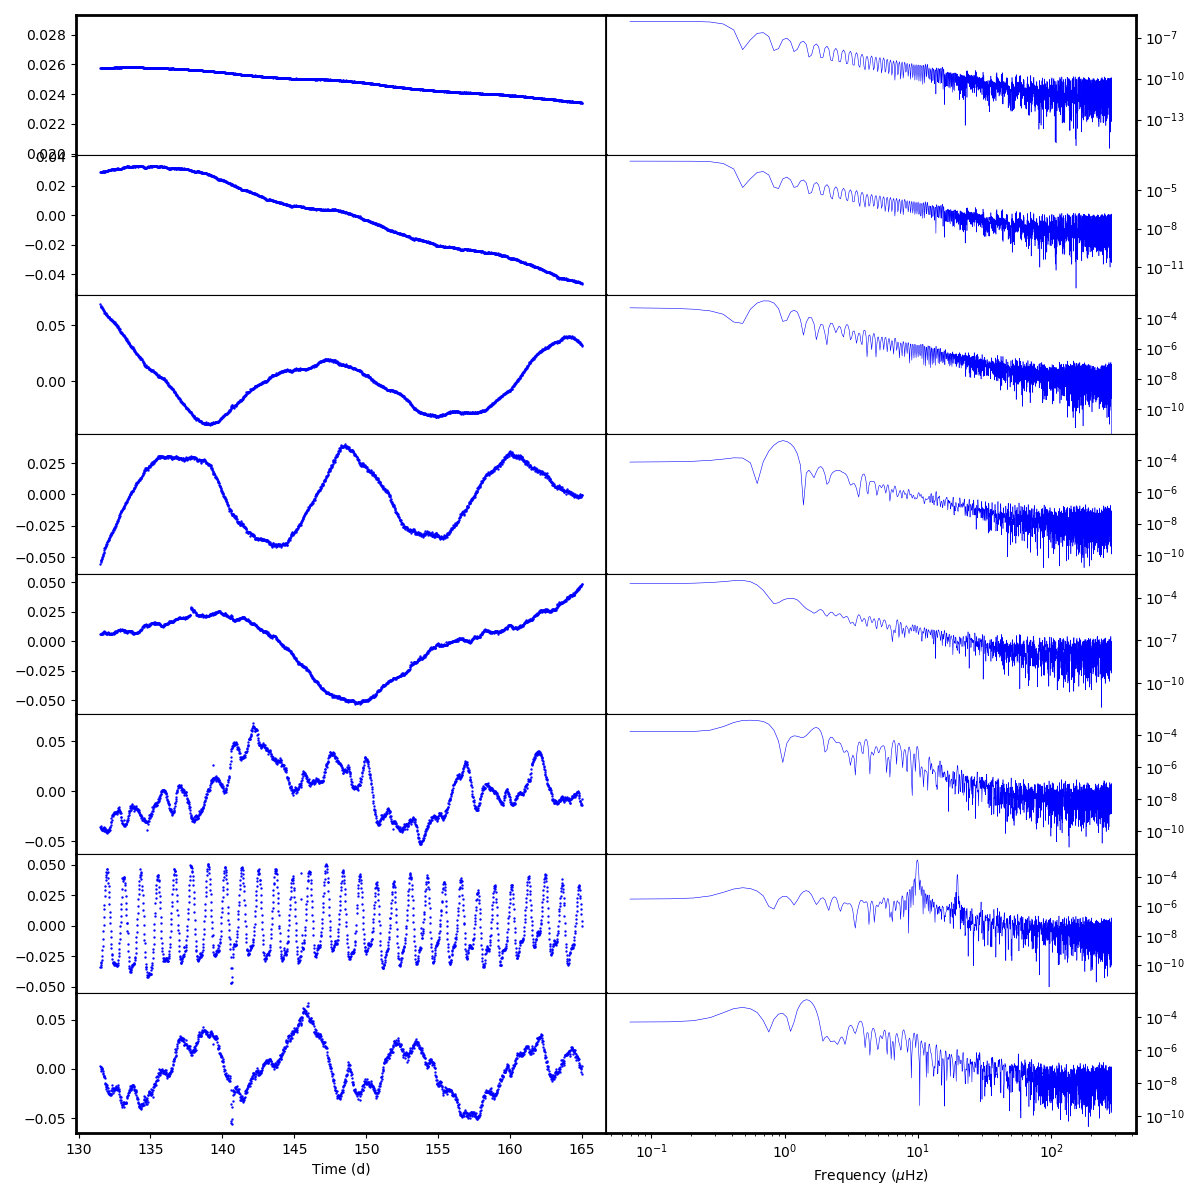
\includegraphics[width=\linewidth]{Chapter5/cbv_6791_q01.png}
    \caption[Custom co-trending basis vectors with Fourier transforms (I) Full image-subtracted subset]{The first 8 co-trending basis vectors (CBVs) for NGC\,6791 for the first data quarter (left), and the Fourier transform of these vectors in log-log space (right) from the full set of image-subtracted light curves.}
    \label{fig:cbvs_allIS_Q1}
\end{figure}

\begin{figure}
    \centering
    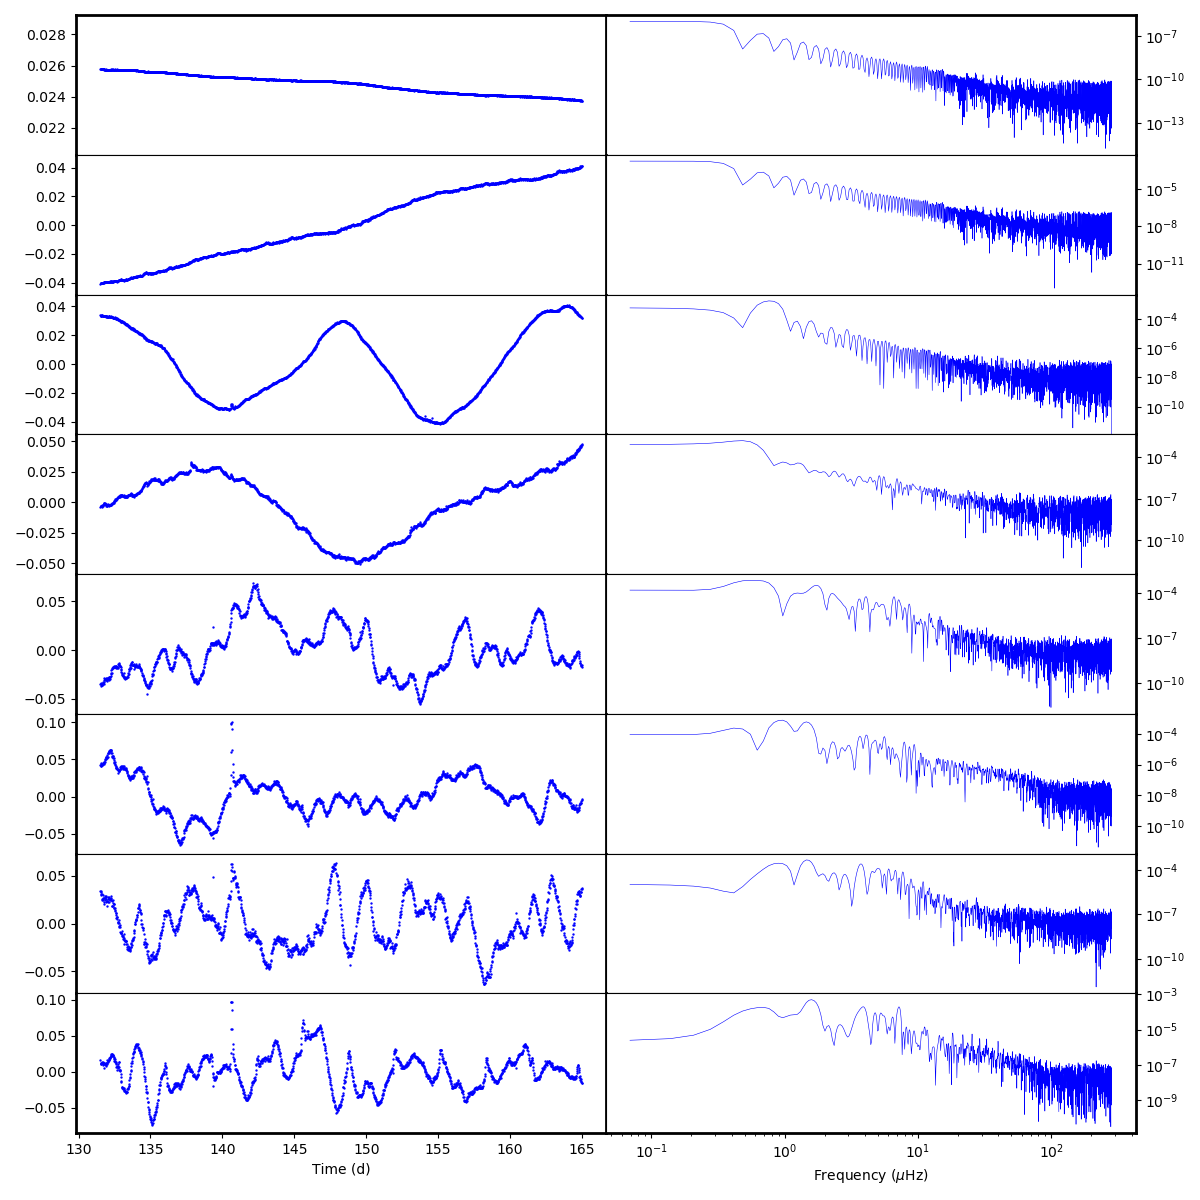
\includegraphics[width=\linewidth]{Chapter5/cbv_6791_rgs_q01.png}
    \caption[Custom co-trending basis vectors with Fourier transforms (II) Red Giant subset]{Same as Figure \ref{fig:cbvs_allIS_Q1} but for the likely red giant member subset of NGC\,6791.}
    \label{fig:cbvs_rgsubset_Q1}
\end{figure}

We implemented a manual correction process that enabled a selected number of CBVs to be applied, based on a least-squares minimisation routine satisfying:

\begin{equation}
    \mathrm{LC}_{\mathrm{corr,n}} = \mathrm{LC}_\mathrm{raw} - \sum_{i=1}^{n} \left(A*\mathrm{CBV}_i + B\right) .
    \label{eqtn:mini}
\end{equation}

\noindent We further designed an automated selection routine that iteratively increased the number of applied CBVs, up to a maximum of 8 vectors, and selected the first corrected light curve where the variance was lower than twice the smallest variance. These selected light curves corrected for the instrumental perturbations, yet retained stellar variability for oscillations above a frequency of about 1\,$\mu$Hz. Figure \ref{fig:cbv_eg_q1} shows the effect of iteratively applying the red giant CBVs to the quarter 1 light curve for KIC\,2436900 in NGC\,6791. We offset the corrected light curves for clarity. We can see that the first CBV removes the predominant low-frequency trend in the light curve (blue to orange), with the application of 3 CBVs correcting for most of the low-frequency variability whilst still retaining the red giant power excess around 30$\mu$Hz, as well as the granulation signal down to a frequency of approximately 3$\mu$Hz. 

\begin{figure}
    \centering
    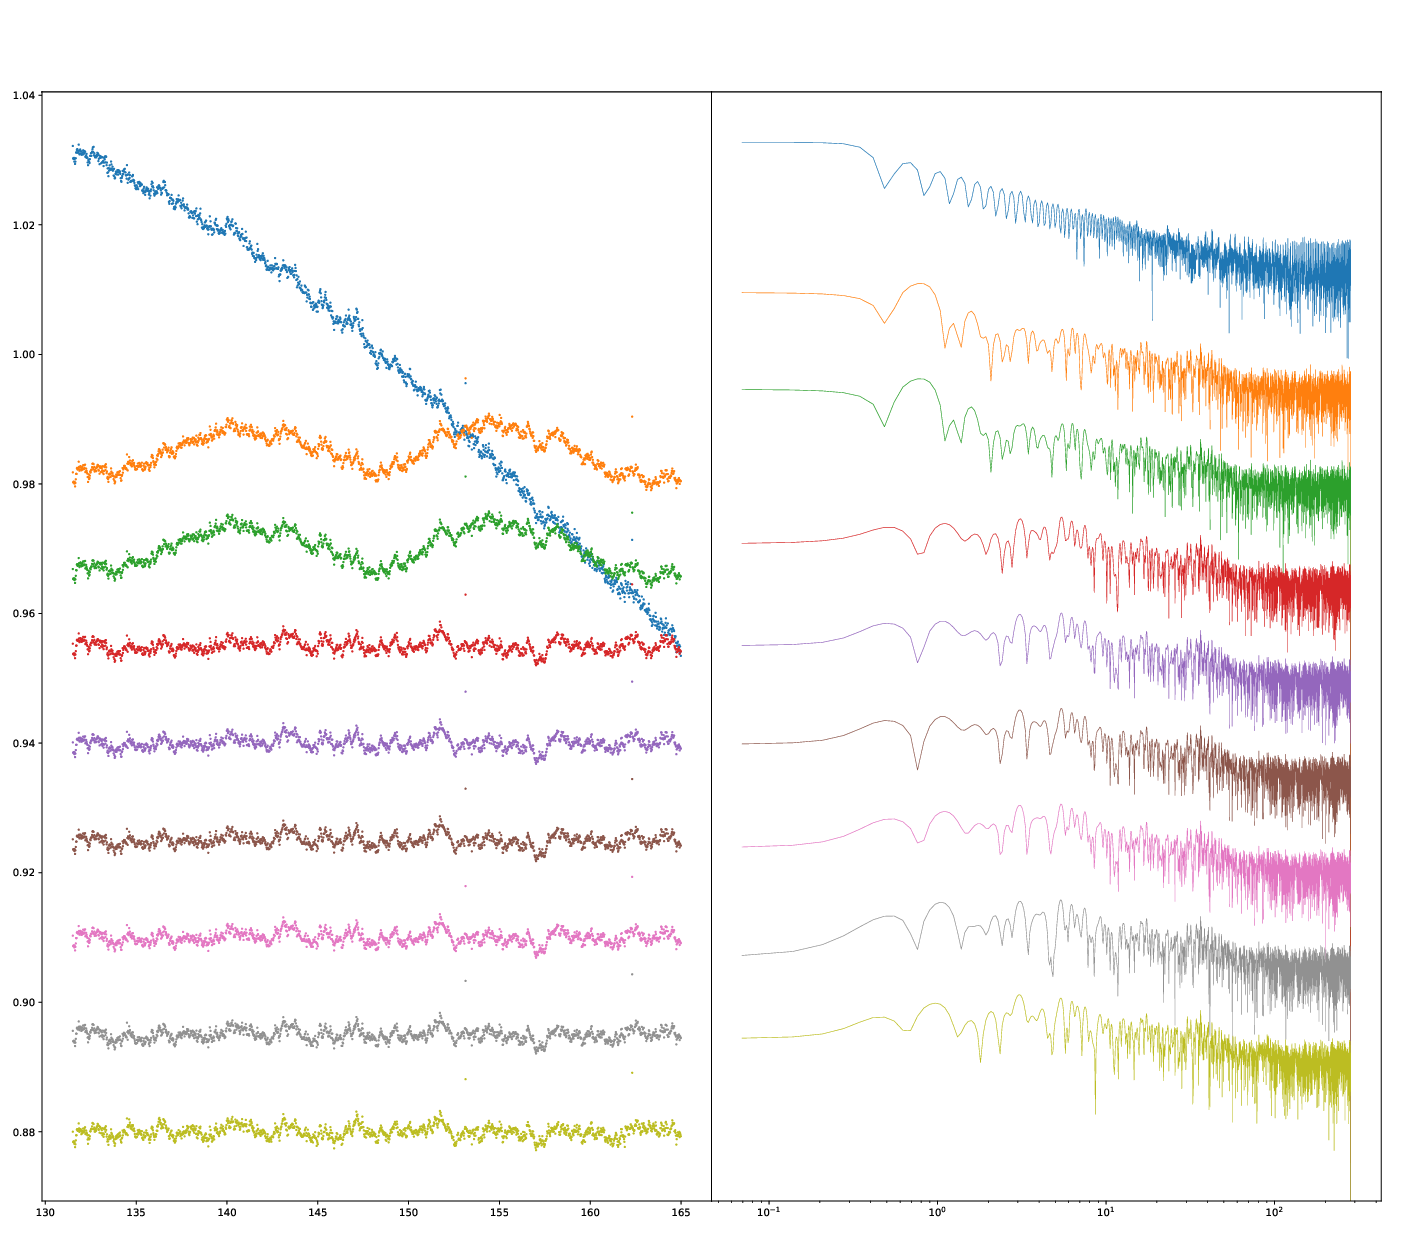
\includegraphics[width=\linewidth]{Chapter5/KIC_2436900_detrending_CBVs_q01_rgs_lsq_mod2.png}
    \caption[Correction effect of applying an increasing number of RG-subset-derived CBVs to a typical RG light curve]{The light curves (left) and power spectra (right) for KIC 2436900 beginning with the raw image-subtracted data (blue), and with increasing orders of applied basis vectors (orange through mustard). The corrected light curves are offset for clarity. Typically, the red corrected light curve would be selected.}
    \label{fig:cbv_eg_q1}
\end{figure}

\subsubsection{Interpolating missing observations}
Further complicating the investigation of low-amplitude oscillations is the window function of the observations \citep{garcia_impact_2014}. Figure \ref{fig:window_function} shows the effect of these time gaps on the spectral window, calculated for a 1\,$\mu$Hz signal with an amplitude of 1\,ppm. The spectral window for the extracted light curves (black) has a very high background level, particularly above 25-30\,$\mu$Hz, due to the introduction of side-lobes of the low-frequency signal at higher frequencies. One of the main causes was \Kepler's angular momentum dumps, which occurred every $\sim3$\,days and resulted in regular gaps of a single long-cadence data point.

\begin{figure}
    \centering
    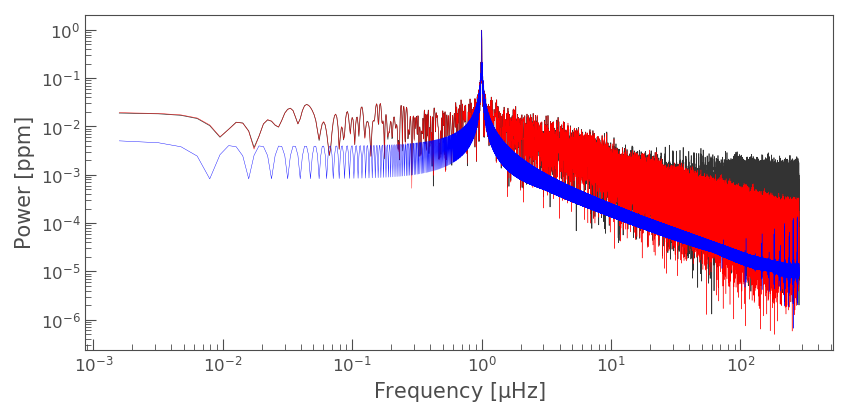
\includegraphics[width=\linewidth]{Chapter5/window_function_example1uHz1ppm.png}
    \caption[Power spectral window, showing the effect of the \Kepler{} window function]{Power spectral window, showing the effect of the \Kepler{} window function on a 1\,ppm 1\,$\mu$Hz signal. The spectral window for the extracted light curves (black line) has a very high background level compared to the same signal observed with the momentum dump gaps interpolated (red signal). For comparison, we have included the power spectrum of the signal observed at a regular cadence with no gaps for the entire \Kepler{} mission (blue line).}
    \label{fig:window_function}
\end{figure}

This spectral window particularly affects the frequency ranges that fainter red giant cluster members oscillate within. To minimize this effect, we interpolated the missing observations from the angular momentum dumps. To interpolate these points we implemented a 5-Fold cross-validated k-Nearest Neighbour (kNN) regression algorithm. The k-Nearest Neighbour algorithm is a simple non-parametric algorithm that selects the `k' data points that are closest to the missing data point in the parameter space, in our case time, and uses the values of these points to predict the missing value. We allow the value of k to vary between 1 and 30 data points for the interpolation, and once again selected our cross-validation sets, to prevent over-fitting, at a 70:30 ratio of training to validation data, with 5 folds. We found that this algorithm almost always selected the 3 closest data points (k=3) to conduct the mean interpolation of flux values for the missing angular momentum dump observations.

Finally, we implemented custom scaling and stitching methods to correct for the quarter to quarter CCD sensitivity differences. Figure \ref{fig:correction_process} presents a summary chart of the correction processes we implemented.

\begin{figure}
    \centering
    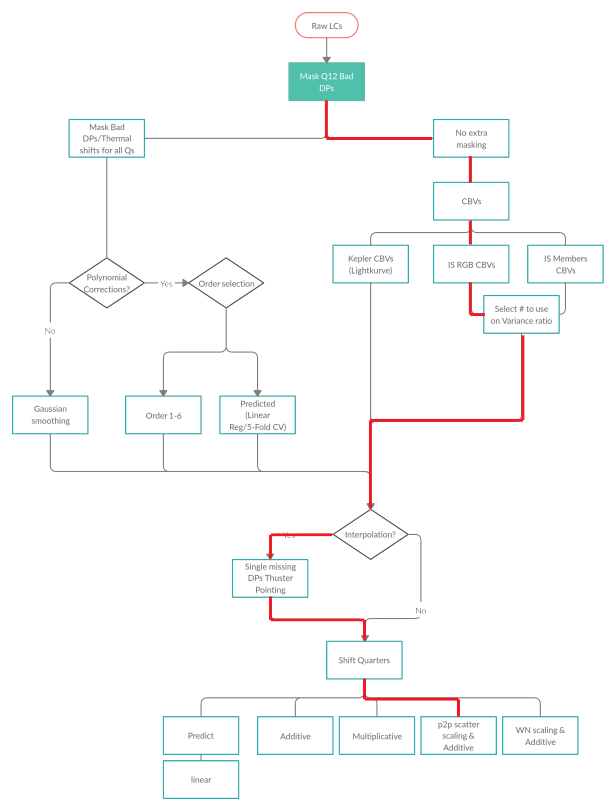
\includegraphics[width=\linewidth]{Chapter5/correction_process.png}
    \caption[Correction process routines]{Flow diagram showing the different correction processes applied to each light curve. The final selected light curve correction routine is highlighted (red line).}
    \label{fig:correction_process}
\end{figure}

\section{Application of Correction methods}

We tested the correction processes on 10 red giants with targeted \Kepler{} light curves of equal length to our image-subtracted light curves. The equal length of observations make these stars ideal test cases. The correction process resulted in over 1\,000 `corrected' light curves with a processing time greater than 15\,minutes per star. These light curves included manual and automated selection of: the number of CBVs applied (to a maximum of 8), and the polynomial order (from 1st order to 6th order corrections), as well as the application of Gaussian high-pass filtering with 0.5\,d, 1\,d and 2\,d kernel widths.

The resulting light curves were then optionally interpolated to fill the single missing observations corresponding to angular momentum dumps. Finally, we stitched the individual quarters together using either an additive or multiplicative flux shift to align the quarters. In the case of the additive flux shift, we also included the option of multiplicative scaling of these quarters based on the point-to-point (p2p) variance, standard deviation, or Lomb-Scargle periodogram white noise amplitude of each quarter.

To speed up the correction process, we processed 10 \Kepler{} targeted red giants with known $\nu_\mathrm{max}$ values and, for each star, manually compared the white noise amplitude and low frequency profiles for our 20 corrected image-subtracted light curves that had the highest signal-to-noise. The automated custom CBVs correction based on the red giant branch subset consistently returned high signal-to-noise ratios of the power excess, as well as retaining more power at low frequencies than Gaussian high-pass filtering. 

For all subsequent red giant light curve corrections, we selected our custom red giant CBV correction routine, interpolated missing points in each quarter using our kNN interpolation method, and finally stitched the resulting light curve quarters with our p2p-scaled additive quarter shift routine. We have marked this process in red in Figure \ref{fig:correction_process}.

We also note that the extracted light curves had a large number of outliers in quarter 12, resulting from coronal mass ejection impacts with \Kepler{} \citep{van_cleve_kepler_2016}, that we removed prior to any other corrections being applied. In the case of those red giants that have a mixture of image-subtracted photometry and simple aperture photometry, we could not assume that our custom CBVs derived from the red-giant subset would accurately correct the systematic perturbations. As such, we only applied a 0.5\,d Gaussian high-pass filter in these cases, to remove the low-frequency trends from each light curve quarter, and then stitched the resulting corrected light curves with our custom p2p-scaled additive shift method.

\subsection{Superstamp times}

During our correction process, we found a small sinusoidal time shift between targeted stars (as downloaded from MAST) and their superstamp light curves (e.g. Figure \ref{fig:keptimediff}). We measured this time shift to have a maximum amplitude of $\sim1.30$\,s for KIC\,2436900 and $\sim1.21$\,s for KIC\,2570924, which are on opposite sides of the superstamp. We attribute this shift to the correction of the observation times to Barycentric Julian Date (BJD). This correction depends on the ecliptic latitude of the specific star, so it varies across the superstamps. For targeted stars these corrections were made individually for each star, but for the superstamps a single correction per cadence was made. We have found that this time shift decreases in amplitude as we move closer to the centre of the \Kepler{} FoV, and infer that these corrections are based on a reference point at its centre. We note this trend for completeness, but due to its negligible effect on our analysis we did not correct for it.

\begin{figure}[h]
    \centering
    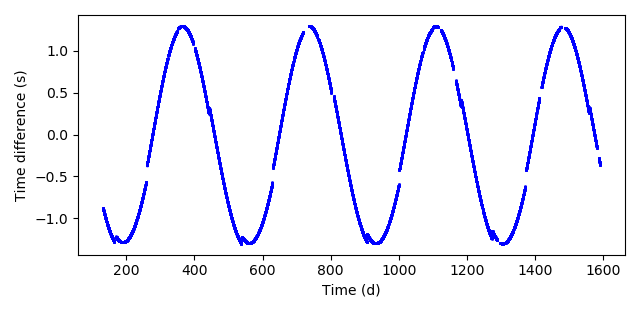
\includegraphics[width=\linewidth]{Chapter5/kepler_time_diff.png}
    \caption[Superstamp and targeted light curve time difference]{Calculated time difference between cadences of the superstamp and targeted light curve for KIC\,2436900.}
    \label{fig:keptimediff}
\end{figure}

\section{Individual results}

We manually reviewed each likely red giant member during our analysis and have identified: 

(a) new red giant members for both NGC\,6791 and NGC\,6819,

(b) rotational modulation in either foreground red dwarfs or background giants, and 

(c) 2 other variable stars. 

Figures \ref{fig:cmd_new} and \ref{fig:cmd_newz} show the CMD for NGC\,6791, based on the likely members from Chapter \ref{chap:membership}, focused on the red giant branch, with the locations of our identified variables marked. Figure \ref{fig:cmd_new_2} shows the same for NGC\,6819.

\begin{figure}
    \centering
    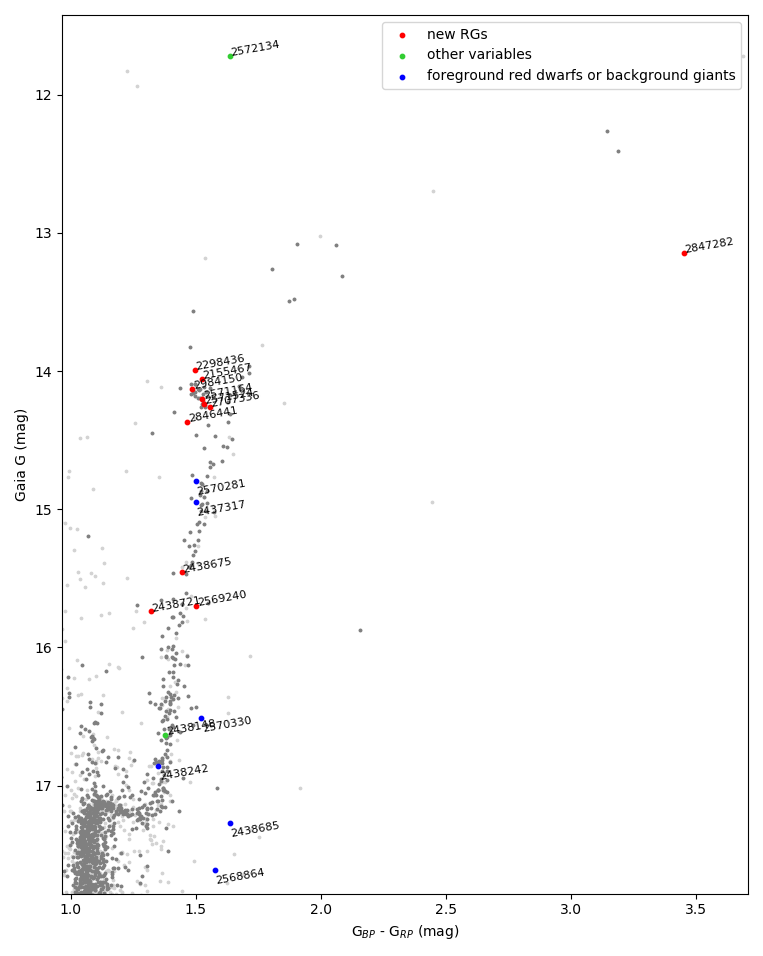
\includegraphics[width=\linewidth]{Chapter5/6791_CMD.png}
    \caption[CMD of new variables in the RG branch in NGC 6791]{CMD of the RG branch in NGC\,6791 with RGs we have identified oscillations in for the first time (red), along with foreground rotational variables (blue), and other interesting variables (green). All likely cluster members (light grey) and the subset of these falling on the \Kepler{} superstamps (dark grey) are shown.}
    \label{fig:cmd_new}
\end{figure}

\begin{figure}
    \centering
    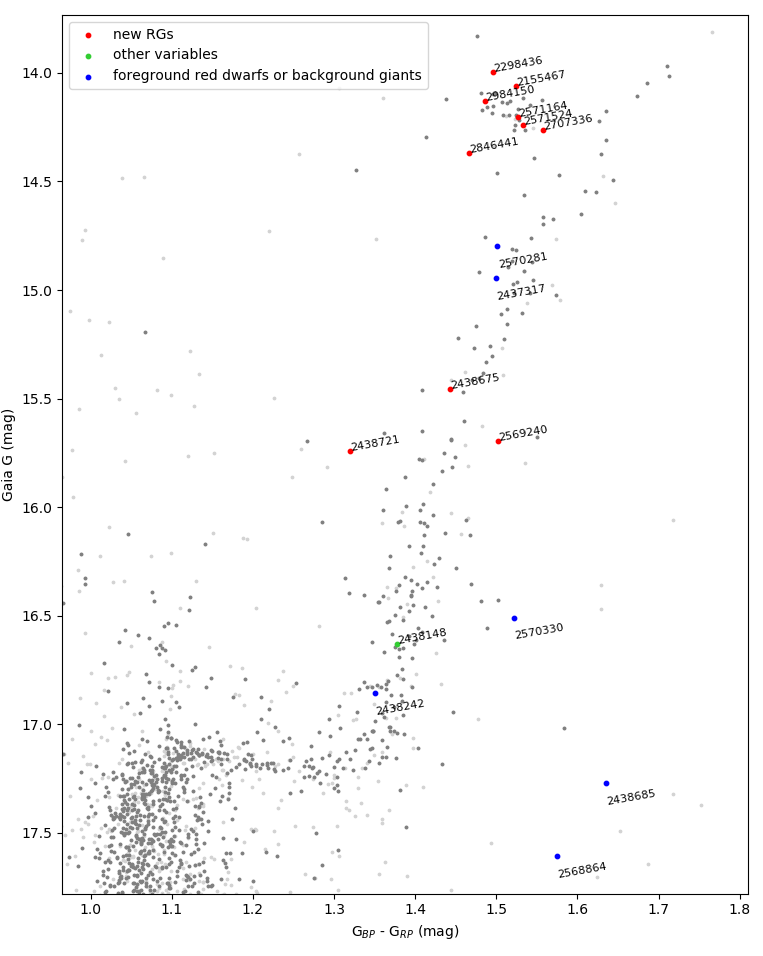
\includegraphics[width=\linewidth]{Chapter5/6791_CMD_zoom.png}
    \caption[NGC\,6791 CMD zoom]{Same as Figure \ref{fig:cmd_new}, zoomed into the crowded region of the RGB.}
    \label{fig:cmd_newz}
\end{figure}


\begin{figure}
    \centering
    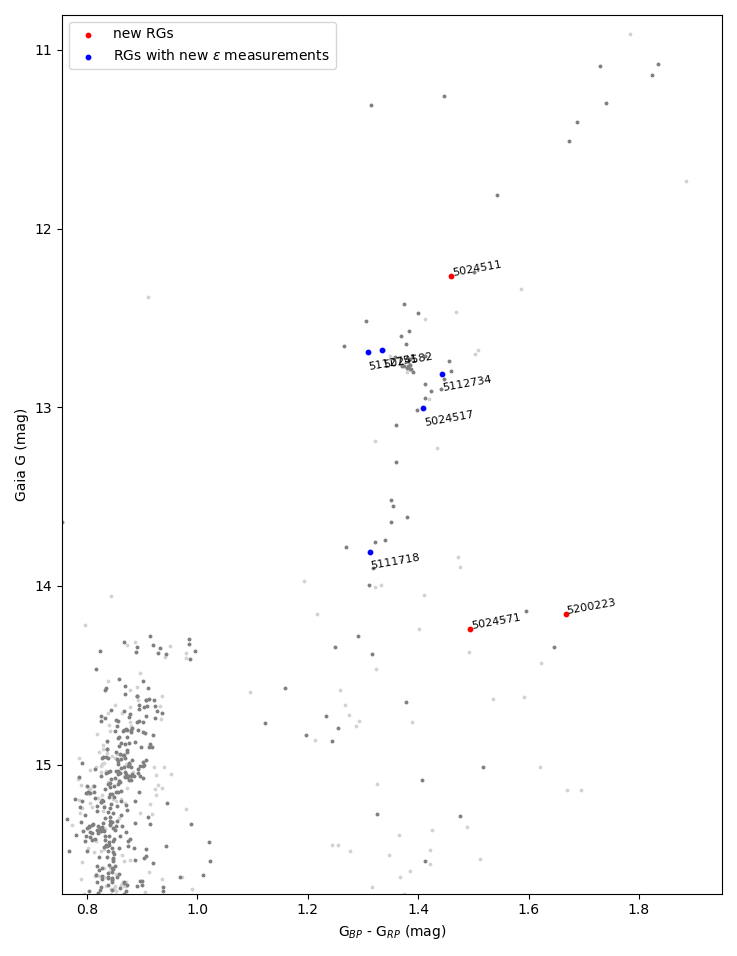
\includegraphics[width=\linewidth]{Chapter5/6819_CMD_newRGS_interesting.png}
    \caption[CMD of new variables in the RG branch in NGC 6819]{CMD of the RG branch in NGC\,6819 with RGs we have identified oscillations in for the first time (red), along with those red giants where we have extracted values for $\epsilon$ for the first time (blue).}
    \label{fig:cmd_new_2}
\end{figure}

\subsection{KIC 2847282}

Figure \ref{fig:2847282_lc} shows the light curve for KIC\,2847282, an M-giant cluster member in NGC\,6791 whose oscillations have not previously been examined in detail. This star does not fall on the \Kepler{} superstamps but was targeted for quarters 10 through 14. In our identification of stellar oscillations in this star we used the \Kepler{} Pre-search Data Conditioning SAP (PDCSAP) \citep{smith_kepler_2012}, a modified version of the simple aperture photometry mentioned in Section \ref{sect:lc_select}, that has been corrected for artefacts such as instrumental systematics. \cite{yu_asteroseismology_2020} included KIC\,2847282 in their ensemble investigation of \Kepler{} long-period variables, noting a period of 27.74\,days but did not identify it as a member of NGC\,6791.

Identification of the centre of the power excess, \numax{}, is difficult in such stars; instead the focus is to identify the individual modes. The power spectrum of KIC\,2847282 is shown in Figure \ref{fig:2847282_ps} (lower panel), with vertical lines marking what are potentially individual oscillation modes, or unresolved groups of modes (one group per radial mode order). These vertical lines connect with the ensemble power spectra from \cite{yu_asteroseismology_2020} (top). We show three potential mode identifications (horizontal lines) based on a cross match between the two plots. Based on the amplitudes, we selected the \numax{} value of 0.68\,$\mu$Hz as corresponding to the most likely mode identifications, with the highest peak corresponding to an order of $n = 2$, with peaks matching up to an order of $n = 5$. We note that the mode identifications corresponding to \numax{} values of $\sim$\,0.41\,$\mu$Hz and $\sim$\,1.0\,$\mu$Hz remain as alternative identifications. This result identifies KIC\,2847282 as the third most luminous red giant in NGC\,6791 and a good candidate for detailed asteroseismic modelling. Whilst we classify this star as a member of NGC\,6791, based on the high membership score (0.72, where any value greater than 0.03 is a likely member), the position of this star in the CMD is unusual for a cluster member, so the possibility exists that this may be a background giant.

\begin{figure}
    \centering
    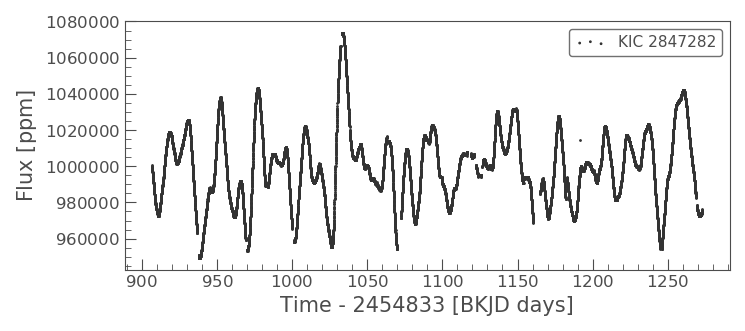
\includegraphics[width=\linewidth]{Chapter5/2847282_MGiant_lc.png}
    \caption[PDCSAP light curve for the new M-giant, KIC\,2847282]{PDCSAP light curve for KIC\,2847282. This is a newly identified M-giant cluster member in NGC\,6791 that does not fall on the superstamps but was targeted for quarters 10 through 14.}
    \label{fig:2847282_lc}
\end{figure}

\begin{figure}
    \centering
    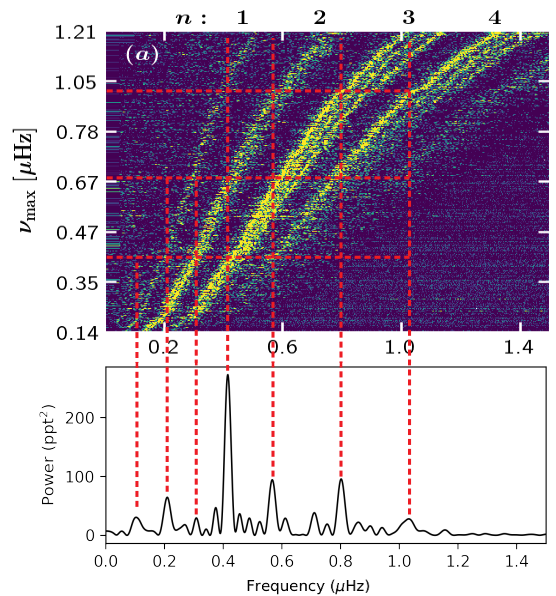
\includegraphics[width=0.6\linewidth]{Chapter5/mode_id_MG.png}
    \caption[Power spectra with possible mode identifications for KIC\,2847282]{Power spectra for KIC\,2847282 (bottom) with three potential values of \numax{} (horizontal lines) based on a cross match between the power spectrum peaks and the ensemble power spectrum trends (top) from \cite{yu_asteroseismology_2020}. The middle line corresponds to our most likely choice of \numax{}$\sim$0.68\,$\mu$Hz, with the highest peak corresponding to an order of n=2, and peak matches up to an order of n=5. The remaining horizontal lines correspond to alternative identifications of \numax{}$\sim$0.41\,$\mu$Hz and \numax{}$\sim$1.0\,$\mu$Hz.}
    \label{fig:2847282_ps}
\end{figure}

\subsection{KIC 5024517}

Figure \ref{fig:5024517_ps} shows the power spectrum for KIC\,5024517, a \Kepler{} target star in NGC\,6819 for which we identify a potential RG\textendash{}RG binary power excess for the first time, centred around $\sim$22$\mu$Hz and $\sim$50$\mu$Hz. It is rare to see a light curve in which oscillations from two red giants are visible. This star was included in \citet{bellamy_using_2015} but only the $\sim$50$\mu$Hz power excess was measured. The decreasing amplitudes of the power excesses with increasing frequency is consistent with two co-distant red giants, with the most likely explanation being that this is a newly identified RG\textendash{}RG binary system. An alternative explanation is this is a blend of two cluster red giants that are located close to each other on the sky. To determine probabilities of red giant line-of-sight blends within the 4” of the Kepler pixels, \citet{colman_pixels_2020} used GALAXIA simulations \citep{sharma_galaxia_2011} to generate artificial populations of stars within a synthesised Kepler FoV. They calculated the occurrence of such alignments to be rare, with a probability of less than 11\%. This occurrence was for a blend between a red giant and any other star. The chance of having two red giants aligned within this distance cutoff is smaller still, although the crowded nature of the cluster means we cannot rule out this possibility without further data. Radial velocity measurements could potentially confirm the possibility of an RG\textendash{}RG binary based on mass ratios if such a system exists.

\begin{figure}
    \centering
    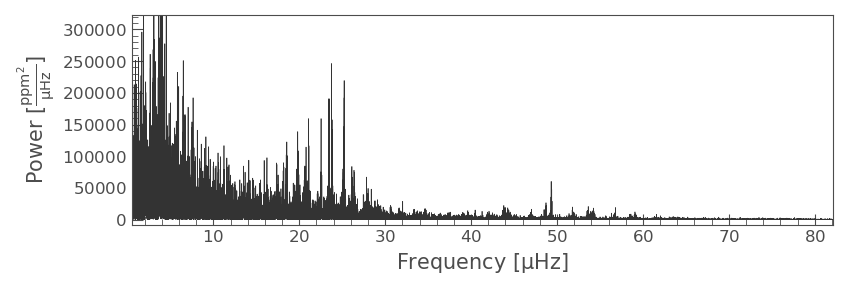
\includegraphics[width=\linewidth]{Chapter5/5024517_ps.png}
    \caption[Power spectrum of the new potential RG\textendash{}RG binary, KIC\,5024517]{Power spectrum of KIC\,5024517, a new potential RG\textendash{}RG binary in NGC\,6819.}
    \label{fig:5024517_ps}
\end{figure}

\subsection{Rotationally-modulated variable stars}

In the course of this work, we re-classified 6 stars in NGC\,6791 from likely red giant members based on our photometric cuts and GMM membership (Chapter \ref{chap:membership}), to either foreground red dwarfs or background giants. Our uncertainty in determining the nature of these stars as either foreground or background stars is due to the unconstrained {\em Gaia} parallax values for each star, with the uncertainty on these values being on order of the value itself. We flagged two of these stars in NGC\,6791, KIC\,2568864 and KIC\,2438685, because their locations in the CMD (Figure \ref{fig:cmd_new}) were too far to the red to be cluster red giants. We inspected their light curves and noted the presence of rotational modulation. Rotational modulation is caused by star spots, providing cooler (and thus dimmer) surface areas that reduce the overall stellar flux, coupled with the stellar rotation period. Such stellar spots in main sequence stars are typically limited in size and change quickly over the timespan of these observations. These light curves are typical of red giants or red dwarf stars, exhibiting stellar flares and rotational modulation. The presence of rotational modulation coupled with the lack of detectable oscillations in the Fourier transforms, and combined with effective temperatures of 4409\,K and 4248\,K, respectively, place these stars as likely foreground red dwarfs, rather than cluster red giants.

The remaining four re-classified stars all fall close to the red giant branch, and for all four we found rotational modulation in their light curves. We note that KIC\,2437317 was previously classified by \cite{bellamy_new_2015} as an M-giant in his Master's thesis \citep{bellamy_using_2015}, however, inspection of the light curve reveals rotational modulation, and the power spectrum shows a resolved peak around 0.31\,$\mu$Hz with a harmonic around 0.62\,$\mu$Hz. In addition, flares are visible in the light curves for KIC\,2437317, around 841.2 and 843.9\,days, and in KIC\,2438242, around 899.3\,days, confirming these stars as M-dwarfs. Figure \ref{fig:reddwarfs} shows the rotational modulation signal evident in the uncorrected quarter 8 and quarter 9 image-subtracted light curves for these stars. The light curves for quarter 9 have been shifted vertically to enable easier comparison of the rotational signal from one quarter to the next. Where possible we measured the rotational periods of these stars using the \texttt{Exoplanet} Gaussian Process code with a simple rotational kernel following the process described in \cite{foreman-mackey_fast_2017}. Table \ref{tab:reclassified} lists the KIC IDs, effective temperatures, alternative ID's from previous photometric studies, and the rotational periods we were able to measured for these reclassified stars. By combining our investigation of the \Kepler{} light curves with our astrometric membership, we were able to improve our cluster membership identifications by removing foreground or background stars that would otherwise have been classified as likely members.

\begin{figure}
    \centering
    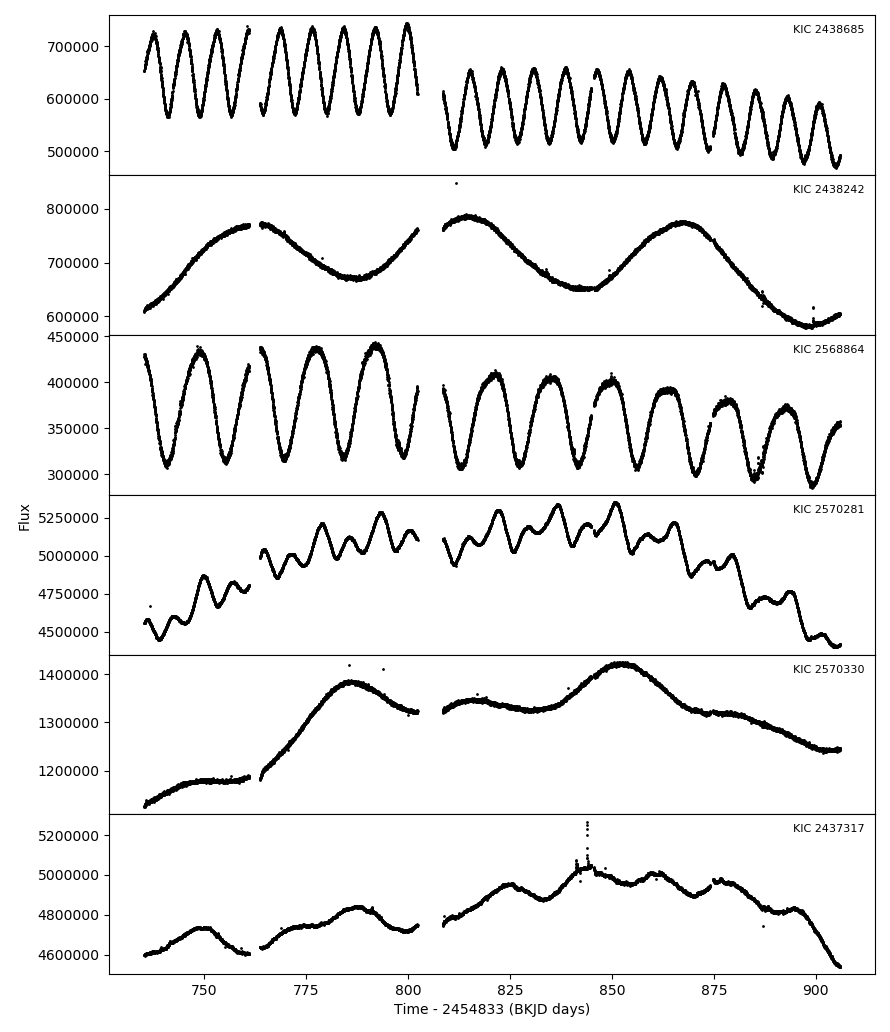
\includegraphics[height=\linewidth]{Chapter5/Rot_mod_5_q89.png}
    \caption[Light curves for 6 re-classified foreground red dwarfs or background giants in NGC 6791]{Light curves for the 6 re-classified foreground red dwarfs or background giants in NGC\,6791, showing characteristic rotational modulation from star spots. KIC\,2437317 shows evidence for flares around 841.2 and 843.9\,days, while KIC\,2438242 shows a potential flare around 899.3\,days. The presence of flares would confirm these stars as M-dwarfs.}
    \label{fig:reddwarfs}
\end{figure}

\begin{table}
    % \centering
    \begin{tabular}{ccccc}
        KIC ID  &   Alternative   & $T_\mathrm{eff}$  & Rotational  & Classification \\%& Reference \\
                &       ID           &    (K)            & Period (d)  &                \\ \hline%& \\ \hline
        2438685 &   \textendash      &  4248             &     7.78    &  \textendash       \\
        2438242 &   V710 Lyr         &  4722             &    54.1     &  M-dwarf \\
        2568864 &   01431\_10        &  4409             &    14.2     &  \textendash       \\%& None\\
        2570281 &   V692 Lyr         &  4643             &    14.5     &  \textendash      \\
        2570330 &   V630 Lyr         &  4609             &    67.7     &  \textendash       \\%& None\\
        2437317 &   V566 Lyr         &  4250             &    17.6     &  M-dwarf     \\

    \end{tabular}
    \caption{Stars re-classified as foreground or background rotational variables}
    \label{tab:reclassified}
\end{table}

\subsection{Other variables}

During inspection of each likely red giant member we identified two other variables in NGC\,6791.  We present the light curves and power spectra for these stars in Figure \ref{fig:weirdvars}. KIC\,2572134 appears to be an irregular variable with a \numax{} around $\sim$6.6\,$\mu$Hz, but it is too blue to be a cluster member unless it is an evolved blue straggler. KIC\,2438148 has a pulsation spectrum that looks typical for a single-mode $\delta$ Scuti variable, but its KIC effective temperature of 4906\,K and colour, $B - V \simeq 1.18$, are too cool for this interpretation. Further investigation, such as obtaining a spectrum, is needed to clarify the variable classification for this star.

\begin{figure}
    \centering
    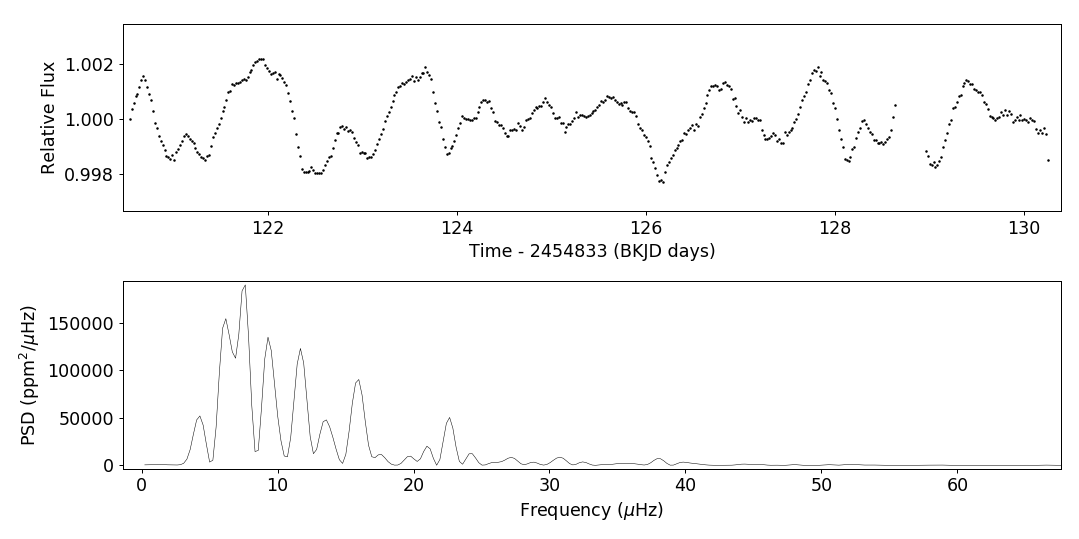
\includegraphics[width=0.9\linewidth]{Chapter5/2572134_lc_ps.png}
    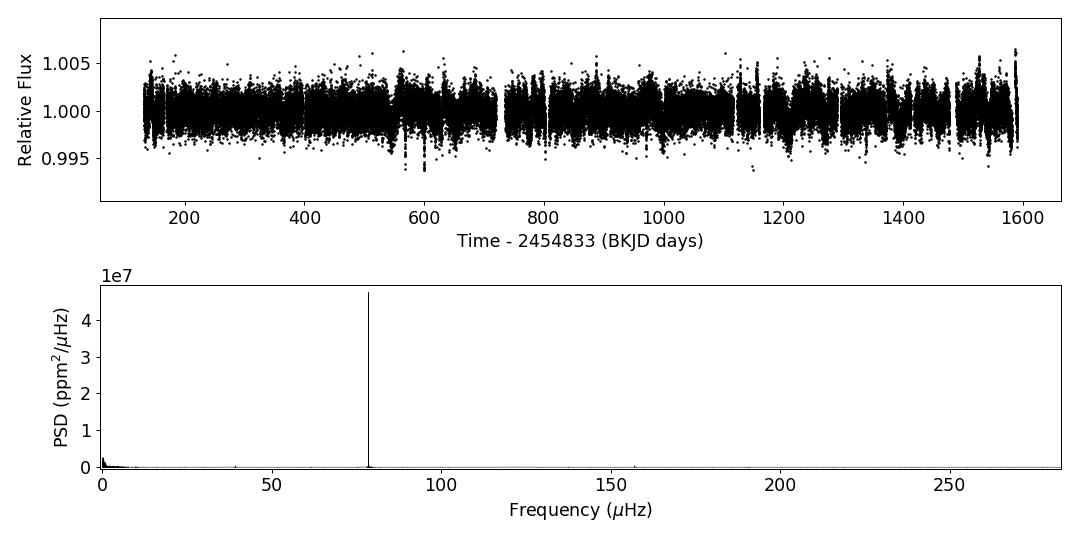
\includegraphics[width=0.9\linewidth]{Chapter5/2438148_lc_ps.png}
    \caption[Light curves and power spectra for KIC\,2572134 and KIC\,2438148]{Light curves and power spectra for KIC\,2572134 (top) and KIC\,2438148 (bottom).}
    \label{fig:weirdvars}
\end{figure}

\section{Ensemble Analysis}

\subsection{Extraction of global parameters}
We have identified 10 and 3 red giants in NGC\,6791 and NGC\,6819, respectively, for which we can now measure oscillation properties for the first time. We used the in-built estimation routines from the \texttt{Lightkurve} package to extract initial estimates of the global asteroseismic parameters, \numax{} and \dnu{}, from the corrected light curves. The \texttt{estimate\_numax} routine uses a 2D auto-correlation function (ACF) to estimate the value of \numax{} from a background corrected power spectrum. Whilst this package can be applied to most red giant oscillators, it is not designed to detect low-frequency oscillations, such as those in high-luminosity red giants. Furthermore, it provides no uncertainty measurement on the \numax{} or \dnu{} values.

To obtain uncertainties on our \numax{} values, we used the \texttt{exoplanet} Gaussian Process (GP) code \citep{foreman-mackey_fast_2017} to simultaneously model the granulation noise and red giant power excess for each light curve. This model relies on an implementation of a \texttt{Celerite} model for asteroseismic modelling with a dual kernel component for modelling stellar granulation, combined with a kernel centred around the \texttt{lightkurve} \numax{} estimate for the red giant power excess, and a constant white noise component. In a few cases, the low signal-to-noise of the excess required a third granulation component to be included for a good fit to be achieved. 

Figure \ref{fig:pm_model} shows an example of a fit of the asteroseismic model to the power excess of KIC\,2437653. The light curve and power spectrum are displayed in the first two panels. The initial fit (middle left) includes the log-scaled power spectrum overlaid with the individual components of the GP model and the complete initial power spectrum fit. The Hamiltonian Monte Carlo (HMC) sampled parameter distribution for the power excess and amplitude are shown (bottom left). We overlaid 100 randomly selected power spectral density trace samples on the original power spectrum (middle right) to highlight the distribution of the fit around \numax{}$\sim$75\,$\mu$\,Hz. Finally, we measured the uncertainty on our \numax{} parameter using a 94\% Highest Posterior Density (HPD) interval in the sampled distribution (bottom right) to account for skewed distributions.

\begin{figure}
    \centering
    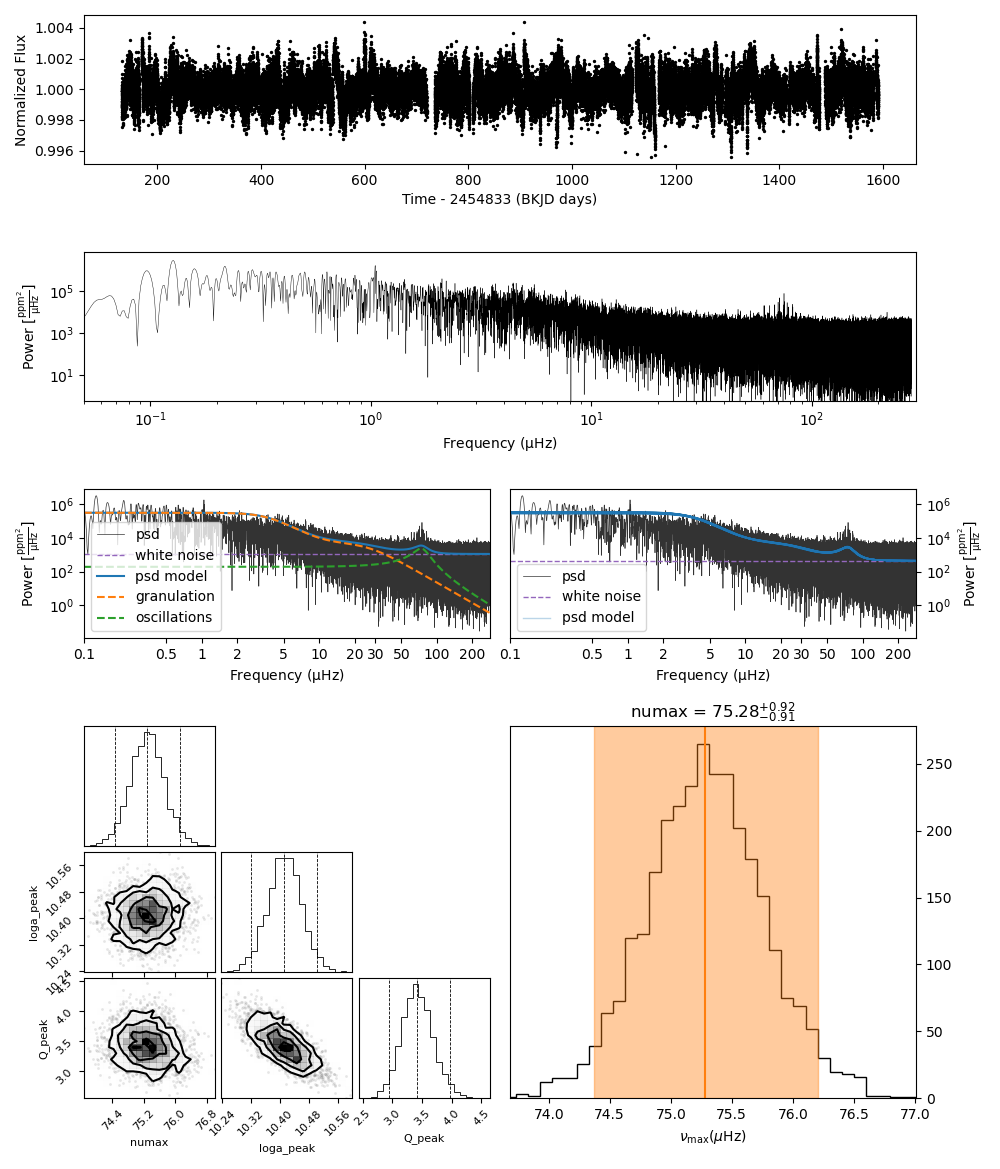
\includegraphics[width=0.95\textwidth]{Chapter5/2437653_pymc3_numax.png}
    \caption[Example of a fit by the asteroseismic GP model for KIC 2437653]{Example of a fit by the asteroseismic GP model for KIC\,2437653. The corrected light curve and resulting power spectrum used in this fit are shown (top two panels). The initial fit (top left) includes the log-scaled power spectrum overlaid with: the two component granulation background (yellow dashed line), the red giant oscillation power excess (green dashed line), white noise (purple dashed line) and the summed model (blue line). The Hamiltonian Monte Carlo (HMC) sampled parameter distribution for the power excess frequency, width, and amplitude, and their correlation, are shown (bottom left), with the distribution of the sampled \numax{} values expanded (bottom right) to highlight the mean value of 75.28\,$\mu$Hz (orange line) and the included uncertainties (orange shaded box). The evaluated power spectral densities for a selection of 100 trace parameter sets is overlaid in blue on the original power spectrum (middle right).}
    \label{fig:pm_model}
\end{figure}

%This has the added benefit of working in the time domain, ... Describe GPs here as well. Whilst this technique should be applicable to extracting deltanu and epsilon we were unable to get this working and have left this extension as future work. For now we have extracted numax for all RGBs with a much lower uncertainty on the extracted/sampled values than can be gained using the Sydney Pipeline. %Due to the memory-intensive nature of this work this was run using the Artemis HPC cluster.

We measured \dnu{} for each red giant by creating interactive \'echelle diagrams with the \texttt{\'Echelle} routine \citep{daniel_hey_echelle_2020}, and selecting the \dnu{} parameter so the $l = 0$ ridge appeared vertical. We then adjusted the value of \dnu{} until the ridge deviated noticeably from vertical and recorded this value as our uncertainty. Finally, we calculated the $\epsilon$ phase shift by measuring the position of the $l = 0$ mode ridge (see \cref{sect:ech}). Figures \ref{fig:echelle_new_6791} and \ref{fig:echelle_new2_6791} show the \'echelle diagrams of each new red giant in NGC\,6791 in which we detected oscillations. Figure~\ref{fig:echelle_new_6819} shows the same for NGC\,6819, with Figure~\ref{fig:echelle_new2_6819} showing \`echelles for red giants identified by \cite{bellamy_using_2015} and which we have created \`echelle diagrams for the first time whilst measuring the phase shift. We present our measured asteroseismic parameters for our newly-identified red giants in Table \ref{tab:6791rgc}, along with two stars we have identified as likely blends, and two stars we present as likely M-giant members, but whose resolution is too low for accurate mode identification to be achieved.

\begin{figure}
    \centering
        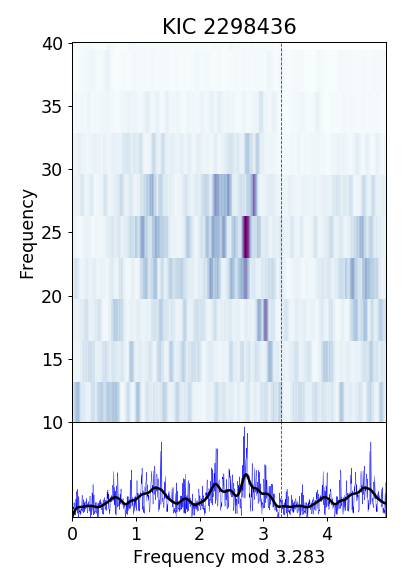
\includegraphics[width=0.3\textwidth]{Chapter5/2298436_echelle.png}
        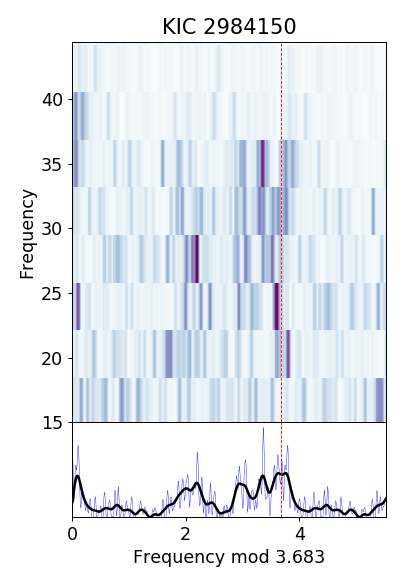
\includegraphics[width=0.3\textwidth]{Chapter5/2984150_echelle.png}
        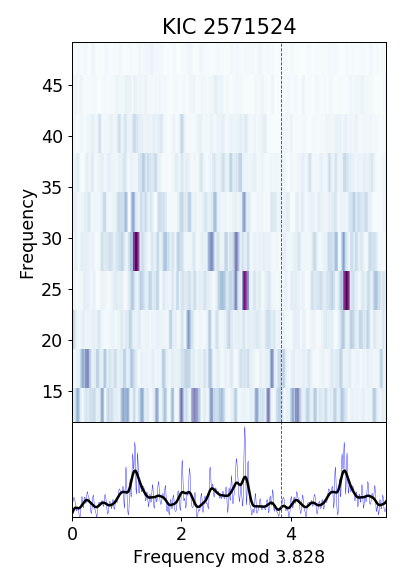
\includegraphics[width=0.3\textwidth]{Chapter5/2571524_echelle.png}
        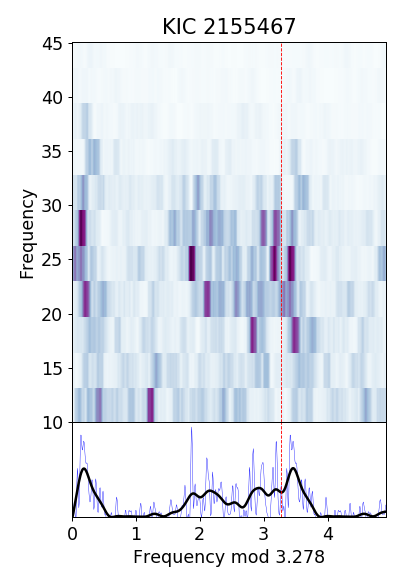
\includegraphics[width=0.3\textwidth]{Chapter5/2155467_echelle.png}
        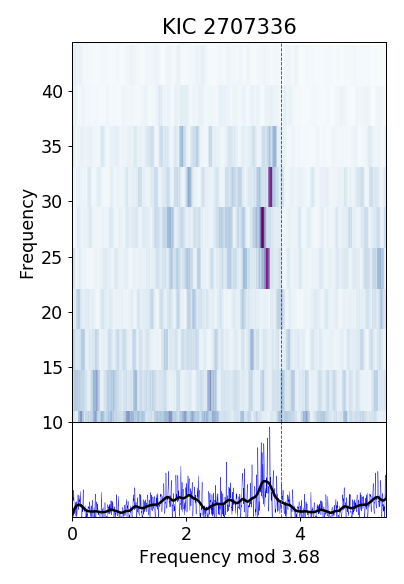
\includegraphics[width=0.3\textwidth]{Chapter5/2707336_echelle.png}
    \caption[\'Echelle diagrams for the newly identified cluster red giants in NGC\,6791 (I)]{\'Echelle diagrams for the newly identified NGC\,6791 red giants, ordered by \numax{}. The red line represents \dnu{} with the \'echelle extended to 1.5 \dnu{} to aid in identifying the $l = 0$ modes when $\epsilon$ is around 1.}
    \label{fig:echelle_new_6791}
\end{figure}

\begin{figure}
    \centering
        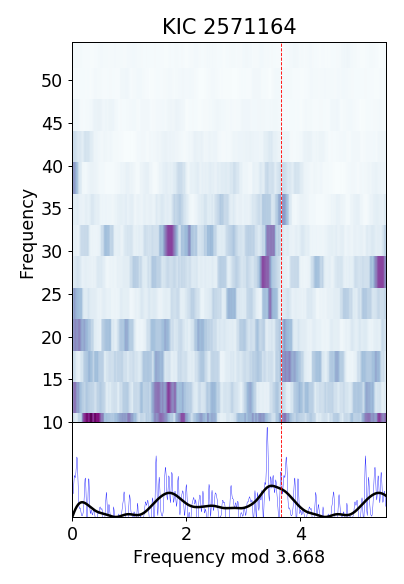
\includegraphics[width=0.3\textwidth]{Chapter5/2571164_echelle.png}
        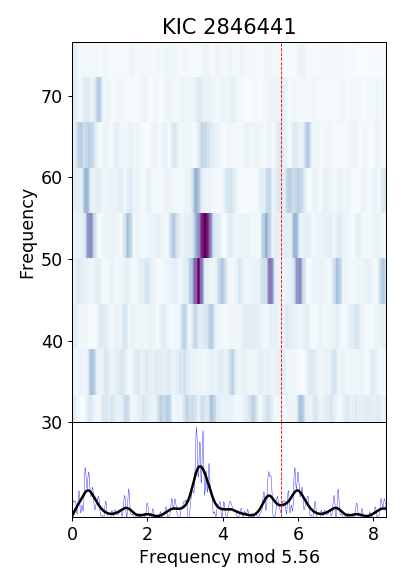
\includegraphics[width=0.3\textwidth]{Chapter5/2846441_echelle.png}
        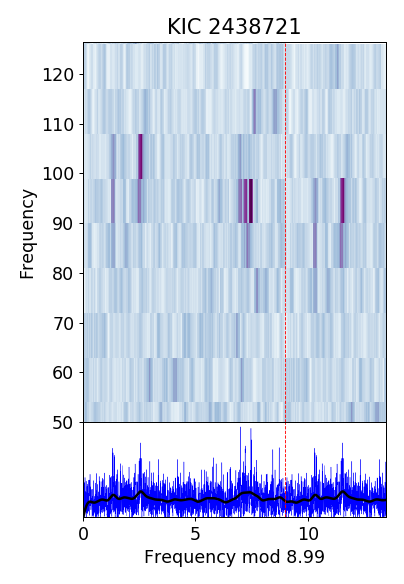
\includegraphics[width=0.3\textwidth]{Chapter5/2438721_echelle.png}
        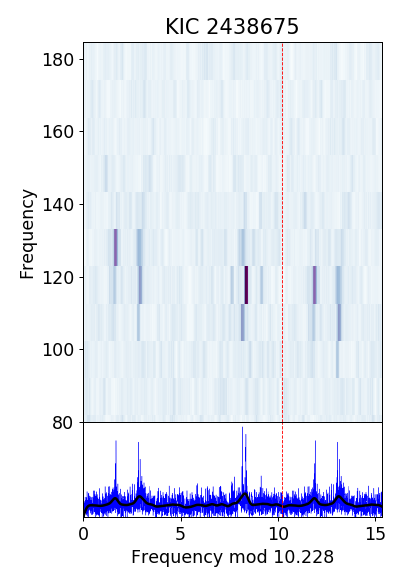
\includegraphics[width=0.3\textwidth]{Chapter5/2438675_echelle.png}
        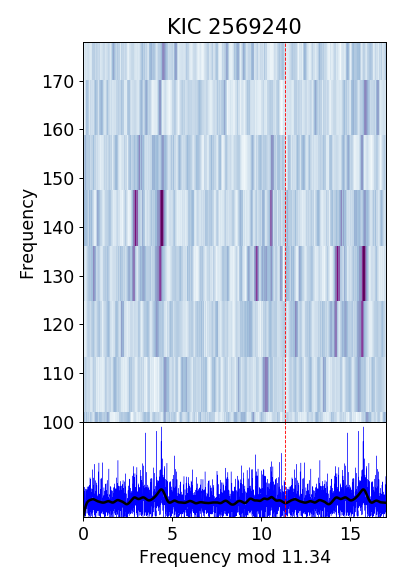
\includegraphics[width=0.3\textwidth]{Chapter5/2569240_echelle.png}
    \caption[\'Echelle diagrams for the newly identified cluster red giants in NGC\,6791 (II)]{Continued from Figure \ref{fig:echelle_new_6791}}
    \label{fig:echelle_new2_6791}
\end{figure}

\begin{figure}
    \centering
        % 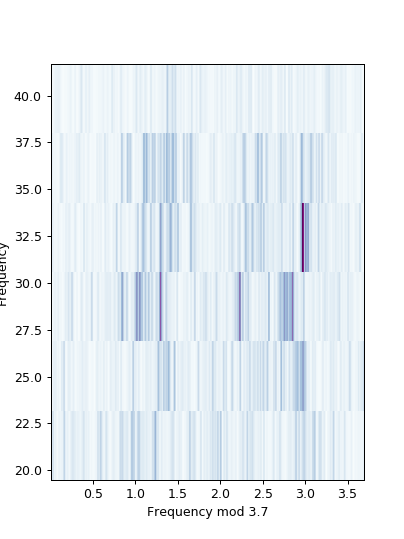
\includegraphics[width=0.32\textwidth]{Chapter5/2437817_echelle_new.png}
        % 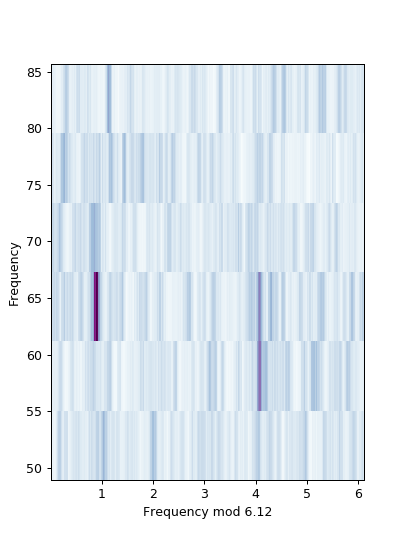
\includegraphics[width=0.32\textwidth]{Chapter5/2438053_echelle_new.png}
        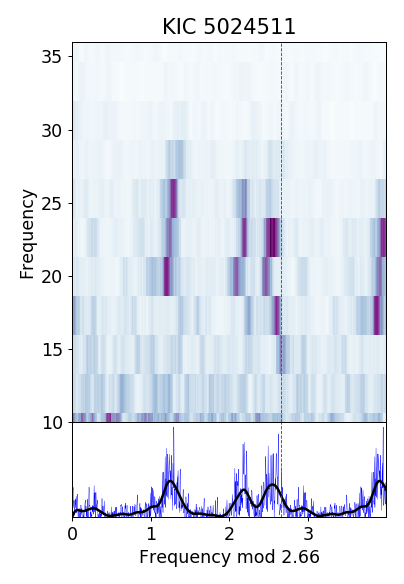
\includegraphics[width=0.32\textwidth]{Chapter5/5024511_echelle.png}
        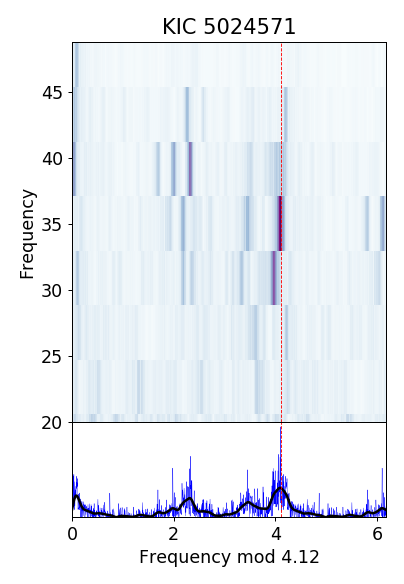
\includegraphics[width=0.32\textwidth]{Chapter5/5024571_echelle.png}
        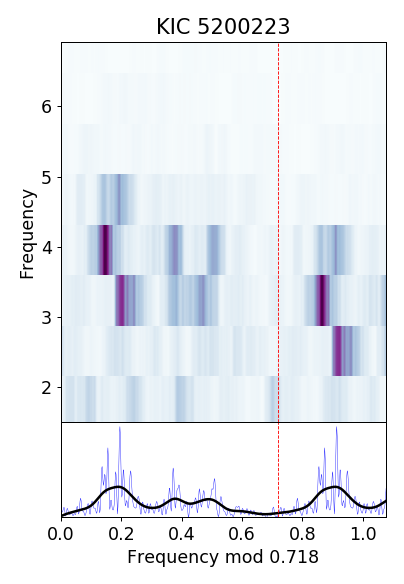
\includegraphics[width=0.32\textwidth]{Chapter5/5200223_echelle.png}
        % 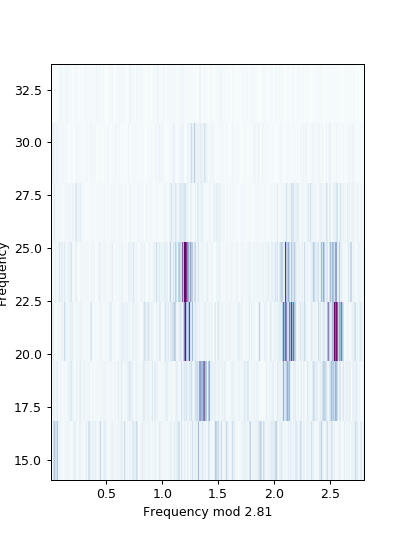
\includegraphics[width=0.32\textwidth]{Chapter5/5025060_echelle_new.png}
    \caption[\'Echelle diagrams for the newly identified cluster red giants in NGC\,6819 (I)]{Same as Figure \ref{fig:echelle_new_6791} but for NGC\,6819.}
    \label{fig:echelle_new_6819}
\end{figure}

\begin{figure}
    \centering
    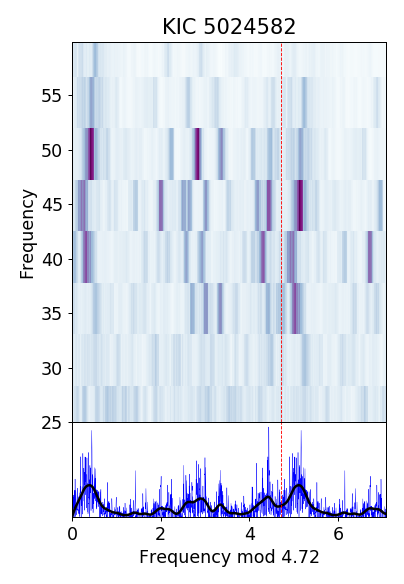
\includegraphics[width=0.32\textwidth]{Chapter5/5024582_echelle.png}
    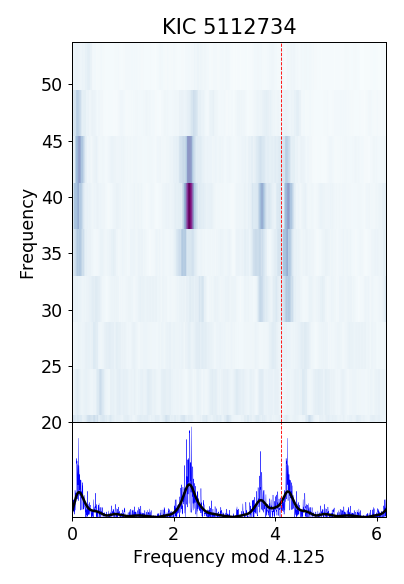
\includegraphics[width=0.32\textwidth]{Chapter5/5112734_echelle.png}
    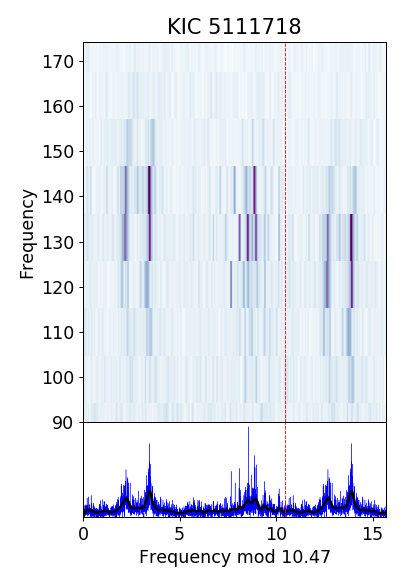
\includegraphics[width=0.32\textwidth]{Chapter5/5111718_echelle.png}
    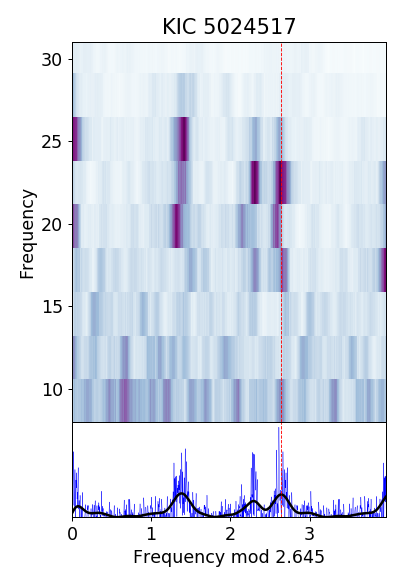
\includegraphics[width=0.32\textwidth]{Chapter5/5024517_a_echelle.png}
    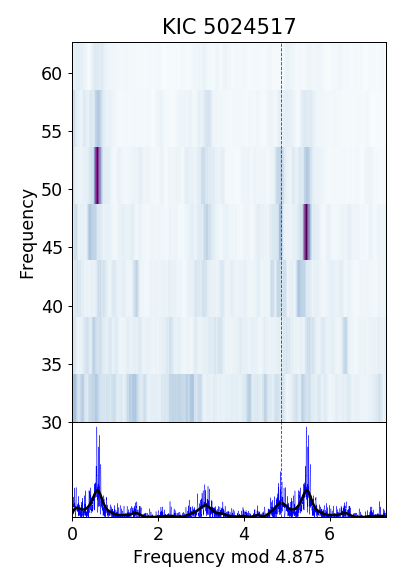
\includegraphics[width=0.32\textwidth]{Chapter5/5024517_b_echelle.png}
    
    \caption[\'Echelle diagrams for the identified cluster red giants in NGC\,6819 (II)]{Same as Figure \ref{fig:echelle_new_6819} for stars identified in Beau Bellamy's thesis \citep{bellamy_using_2015}, that we have produced \`echelle diagrams for, for the first time. The last two panels show individual \`echelle diagrams for the two red giant power excesses we have identified in KIC\,5024517.}
    \label{fig:echelle_new2_6819}
\end{figure}

\begin{table}
    \centering
    \setlength\tabcolsep{10pt}
    \resizebox{\textwidth}{!}{%
        \begin{tabular}{cccccccccccccccccl}
            \toprule
            KIC ID	&	NGC		&  meanprob	&K$_\mathrm{p}$ &	\numax{}	&	GP $\nu_{\mathrm{max}}$	&	\dnu{}	&	$\sigma_{\Delta\nu}$	&	$\epsilon$	&	Notes	\\
            \midrule
            2847282 &   6791    &   0.721   &   8.34        &   0.68        &         \textemdash       &\textemdash&   \textemdash     &  \textemdash& New M-giant \\
            2155467	&	6791	&	0.899	&	14.08		&	30.14		&  26.78$^{+0.63}_{-0.61}$  &	3.28	&		0.05		&	1.06	&	\\
            2298436	&	6791	&	0.903	&	14.02		&	28.87		&  26.07$^{+0.45}_{-0.39}$ &	3.28	&		0.07		&	0.84	&	\\
            2438675	&	6791	&	0.950	&	15.47		&	117.9		&         \textemdash       &	10.23	&		0.03		&	1.28	&	\\
            2438721	&	6791	&	0.789	&	15.75		&	97.26		&112.29$^{+27.52}_{-26.57}$	&	8.99	&		0.03		&	1.28	&	\\
            2569240	&	6791	&	0.964	&	15.71		&	137.46		&         \textemdash       &	11.34	&		0.08		&	1.39	&	\\
            2571164	&	6791	&	0.896	&	14.20		&	34.88		&  32.39$^{+1.05}_{-1.13}$	&	3.67	&		0.10	    &	0.95	&	\\
            2571524	&	6791	&	0.744	&	14.25		&	29.69		&  31.50$^{+0.98}_{-0.90}$  &	3.83	&		0.10		&	0.83	&	\\
            2707336	&	6791	&	0.924	&	14.30		&	33.55		&  31.31$^{+0.64}_{-0.61}$  &	3.68	&		0.10	    &	0.93	&	\\
            2846441	&	6791	&	0.744	&	14.41		&	56.81		&  54.17$^{+1.67}_{-1.89}$  &	5.56	&		0.20	    &	1.08	&	\\
            2984150	&	6791	&	0.620	&	14.19		&	29.32		&  31.35$^{+0.78}_{-0.71}$  &	3.68	&		0.10	    &	1.02	&	\\
            \midrule
            2437817	&	6791	&	0.967	&	16.54		&	32.19		&         \textemdash       &	3.7		&		0.20		&	0.80	&	Likely blend with KIC\,2437805\\
            2438053	&	6791	&	0.964	&	16.49		&	58.93		&         \textemdash       &	6.13	&		0.02		&	0.66	&	Likely blend with KIC\,2438038\\
            \midrule
            5024511	&	6819	&	0.147	&	12.31		&	24.43		&  31.65$^{+0.64}_{-0.88}$  &	2.66	&		0.20		&	0.95	&	RG light curve has contamination from $\delta$ Scuti\\
            5024571	&	6819	&	0.773	&	14.28		&	39.13		&         \textemdash       &	4.12	&		0.10	    &	0.99	&	RG light curve has contamination from $\delta$ Scuti\\
            5200223	&	6819	&	0.294	&	14.19		&	3.77		&						    &	0.71	&		0.05		&	0.72	&	\\
            \midrule
            5024582	&	6819	&	0.304	&	10.30		&	46.44		&         \textemdash       &	4.72	&		0.10		&	1.07	&	New \dnu{} and $\epsilon$ measurements\\
            5112734	&	6819	&	0.961	&	10.20		&	41.19		&         \textemdash       &	4.12	&		0.10		&	1.04	&	New \dnu{} and $\epsilon$ measurements\\
            5111718	&	6819	&	0.818	&	11.48		&	134.2		&         \textemdash       &	10.47	&		0.20		&	1.33	&	New \dnu{} and $\epsilon$ measurements\\
        5024517 (A)	&	6819	&	0.960	&	9.62		&	23.35		&         \textemdash       &	4.88	&		0.10		&	1.02	&	New \dnu{} and $\epsilon$ measurements\\
        5024517 (B)	&	6819	&	0.960	&	9.62		&	50.72		&         \textemdash       &	2.65	&		0.10		&	1.00	&	New \dnu{} and $\epsilon$ measurements\\
            5112751	&	6819	&	0.915	&	10.34		&	84.73		&         \textemdash       &	6.18	&		0.10		&	1.03	&	New \dnu{} and $\epsilon$ measurements\\
            \midrule
            5112483	&	6819	&	0.433	&	11.24		&\textemdash	&         \textemdash       &\textemdash&   \textemdash	&\textemdash	&	Likely M-Giant from LC. Resolution too low for order matching.\\
            5200056	&	6819	&	0.639	&	10.88		&\textemdash	&         \textemdash       &\textemdash&   \textemdash	&\textemdash	&	Likely M-Giant from LC. Resolution too low for order matching.\\

            \bottomrule
        \end{tabular}
    }
    \caption[List of newly identified red giants]{List of newly identified red giants from this work. GP \numax{} values are not available for KIC\,2438675 and KIC\,2569240 as the signal-to-noise of the red giant excess was too low to obtain a constrained fit, while in KIC\,5024571, the contaminating $\delta$ Scuti oscillations prevented the GP model from converging. GP \numax{} values were not calculated for the RGs identified by Beau Bellamy in his Masters' thesis \citep{bellamy_using_2015}, these are included to present our new $\epsilon$ and \dnu{} measurements only.}
    \label{tab:6791rgc}
\end{table}

\section{Asteroseismic Diagrams}

For large ensemble asteroseismic analyses, we must reduce stellar spectra to a few measurable parameters that describe fundamental stellar properties. These parameters for solar-like oscillators include \numax{}, \dnu{}, and $\epsilon$. Asteroseismic diagrams provide an intuitive format for investigating the relationships between these parameters and their corresponding connection to the intrinsic stellar properties. In the case of open clusters, where populations are considered to be coeval and co-metallic, we have ideal ensembles for investigating stellar evolutionary tracks and thus the function of stellar mass in these diagrams. These functions can then be applied to larger samples where age or metallicity may be unknown. We present cluster red giants on the same \numax{} \textendash{} \dnu{} and \dnu{} \textendash{} $\epsilon$ diagrams as the entire \Kepler{} sample for the first time, effectively presenting empirical isochrones based on the homogeneous cluster properties. Hereafter, we refer to these empirical isochrones showing tight relationships in \numax{}, $\Delta\nu$, $\epsilon$, and photometric magnitudes as isochrones.

We combined the red giant samples from \cite{hon_deep_2018}, \cite{yu_asteroseismology_2018-1} and \cite{yu_asteroseismology_2020}, as well as red giants from Beau Bellamy's Masters' thesis \citep{bellamy_using_2015}, to produce a complete sample of previously studied red giants in the nominal \Kepler{} FoV, henceforth referred to as the field star sample. We then cross-matched this sample with our likely red giant cluster membership lists to isolate the studied cluster red giants for NGC\,6791 and NGC\,6819. We note that \numax{} and \dnu{} for all of the red giants in \cite{hon_deep_2018} have also been extracted by either \cite{yu_asteroseismology_2018-1} or \cite{yu_asteroseismology_2020}. Yu et al.'s combined sample (Yu) is slightly larger than that of \cite{hon_deep_2018} for the cluster red giants, so we selected their values for these parameters for consistency. By combining the results from Yu, and Bellamy, with our new detections, we obtained determinations for \numax{} and \dnu{} for 150 and 131 stars in NGC\,6791 and NGC\,6819, respectively.

\cite{stello_asteroseismic_2011} have shown that cluster red giants show a tight relationship between apparent magnitude and their asteroseismic parameters of \numax{} and \dnu{}. This is a result of the similar masses and effective temperatures shared by red giant cluster members. The luminosity differences between cluster members is therefore the dominant factor affecting these values, which corresponds to apparent magnitude for cluster members because they are effectively co-distant. \cite{stello_detection_2010} and \cite{bellamy_new_2015} have shown that this relationship can be used for asteroseismic cluster membership determinations. Figure \ref{fig:magdnu} shows the $K$ mag vs \dnu{} relation for the clusters of NGC\,6791 and NGC\,6819. The cluster members of single isolated stars are clearly delineated into isochrones, with the red clumps visible just above the RGB sequences around \numax{}$\sim$30\,$\mu$Hz and $\Delta\nu\sim$3.8$\mu$Hz. 

We identified 46 and 21 outliers for the NGC\,6791 and NGC\,6819 ensembles, respectively, which were classified in Beau Bellamy's thesis as likely members. We reclassify these stars as likely non-members based on this diagram although a small fraction could be exotic stars arising from interactions with other stars. Our membership analysis does not account for binary systems, making a numerical estimate of the likelihood of membership for these stars difficult, although future Gaia releases should have the ability to distinguish binary stars based on astrometric excess noise \citep{gandhi_astrometric_2020}. This will provide future analyses with the option of dividing the dataset into multiple stellar systems and single star systems prior to clustering, allowing us to identify and account for kinematic deviations from the average cluster values, arising from the motion of binaries. The possibility of even a small fraction of these stars being members with exotic interaction histories makes these interesting targets for follow up investigations. 

We also note the presence of 2 potential evolved blue stragglers in NGC\,6791, lying about 0.75\,mag above the isochrone in the $K$ mag \textendash \dnu{} diagram. We categorise these stars as potential evolved BSs as they both have high membership scores, so are very likely cluster members, and have magnitudes with an offset of 0.75\,mag from the empirical cluster isochrone, corresponding to the maximum offset expected from a binary merger between 2 equal mass stars. Binary merger products often appear on or near the main sequence, to the blue of the cluster's main-sequence turnoff point. Such stars are called blue stragglers and as these stars evolve off the main sequence they remain blue of the red giant branch, where they are referred to as evolved blue stragglers. KIC\,5025717 also lies within this same magnitude range of the empirical cluster isochrone for NGC\,6819. Whilst it falls outside the \Kepler{} superstamps it was targeted in the nominal mission, and all three stars exhibit red giant power excesses \citep{yu_asteroseismology_2016}. Figure \ref{fig:ebss} presents PDCSAP-based amplitude spectra we have extracted from these nominal \Kepler{} targets. It is possible other evolved blue stragglers could also be present in this sample with smaller magnitude offsets from non-equal mass mergers, although such an investigation is beyond the scope of the current work.

\begin{figure}
    \centering
    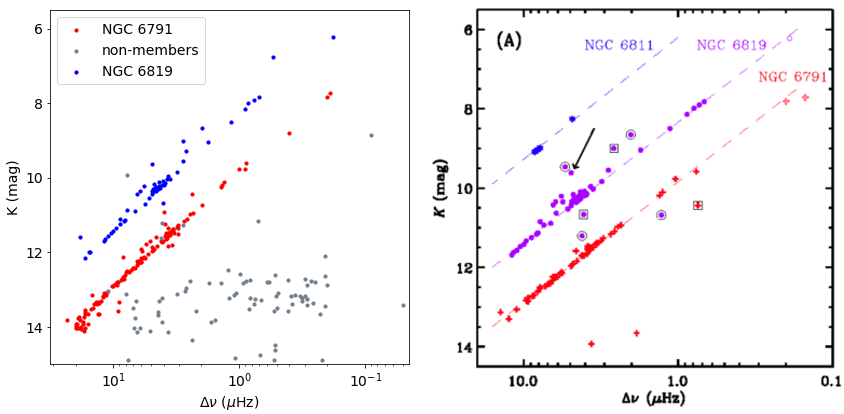
\includegraphics[width=\linewidth]{Chapter5/kmag-dnu-both.png}
    % 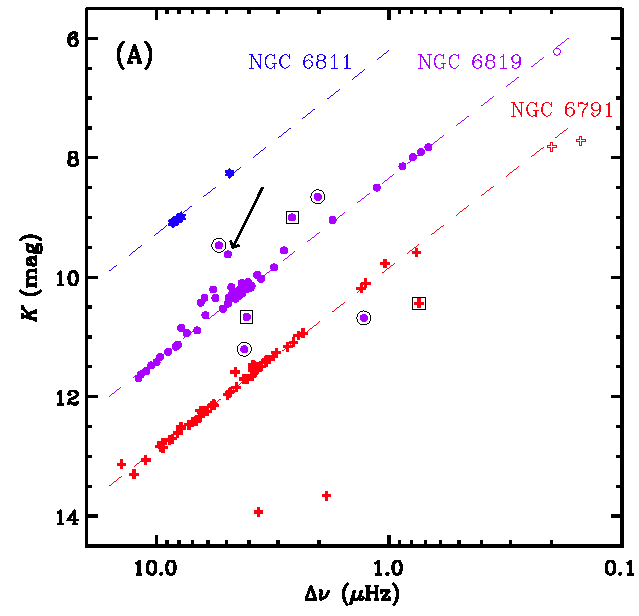
\includegraphics[width=0.48\linewidth]{Chapter5/stello_11_kmagdnu.png}
    \caption[$K$mag \textendash \dnu{} relation for NGC\,6791 and NGC\,6819]{$K$mag \textendash \dnu{} relation for NGC\,6791 (red) and NGC\,6819 (blue), with outliers (grey) from our compiled database (left) and the corresponding diagram from \citep{stello_asteroseismic_2011} (right). Outliers (grey) may include exotic cluster members such as mergers.}
    \label{fig:magdnu}
\end{figure}

\begin{figure}
    \centering
    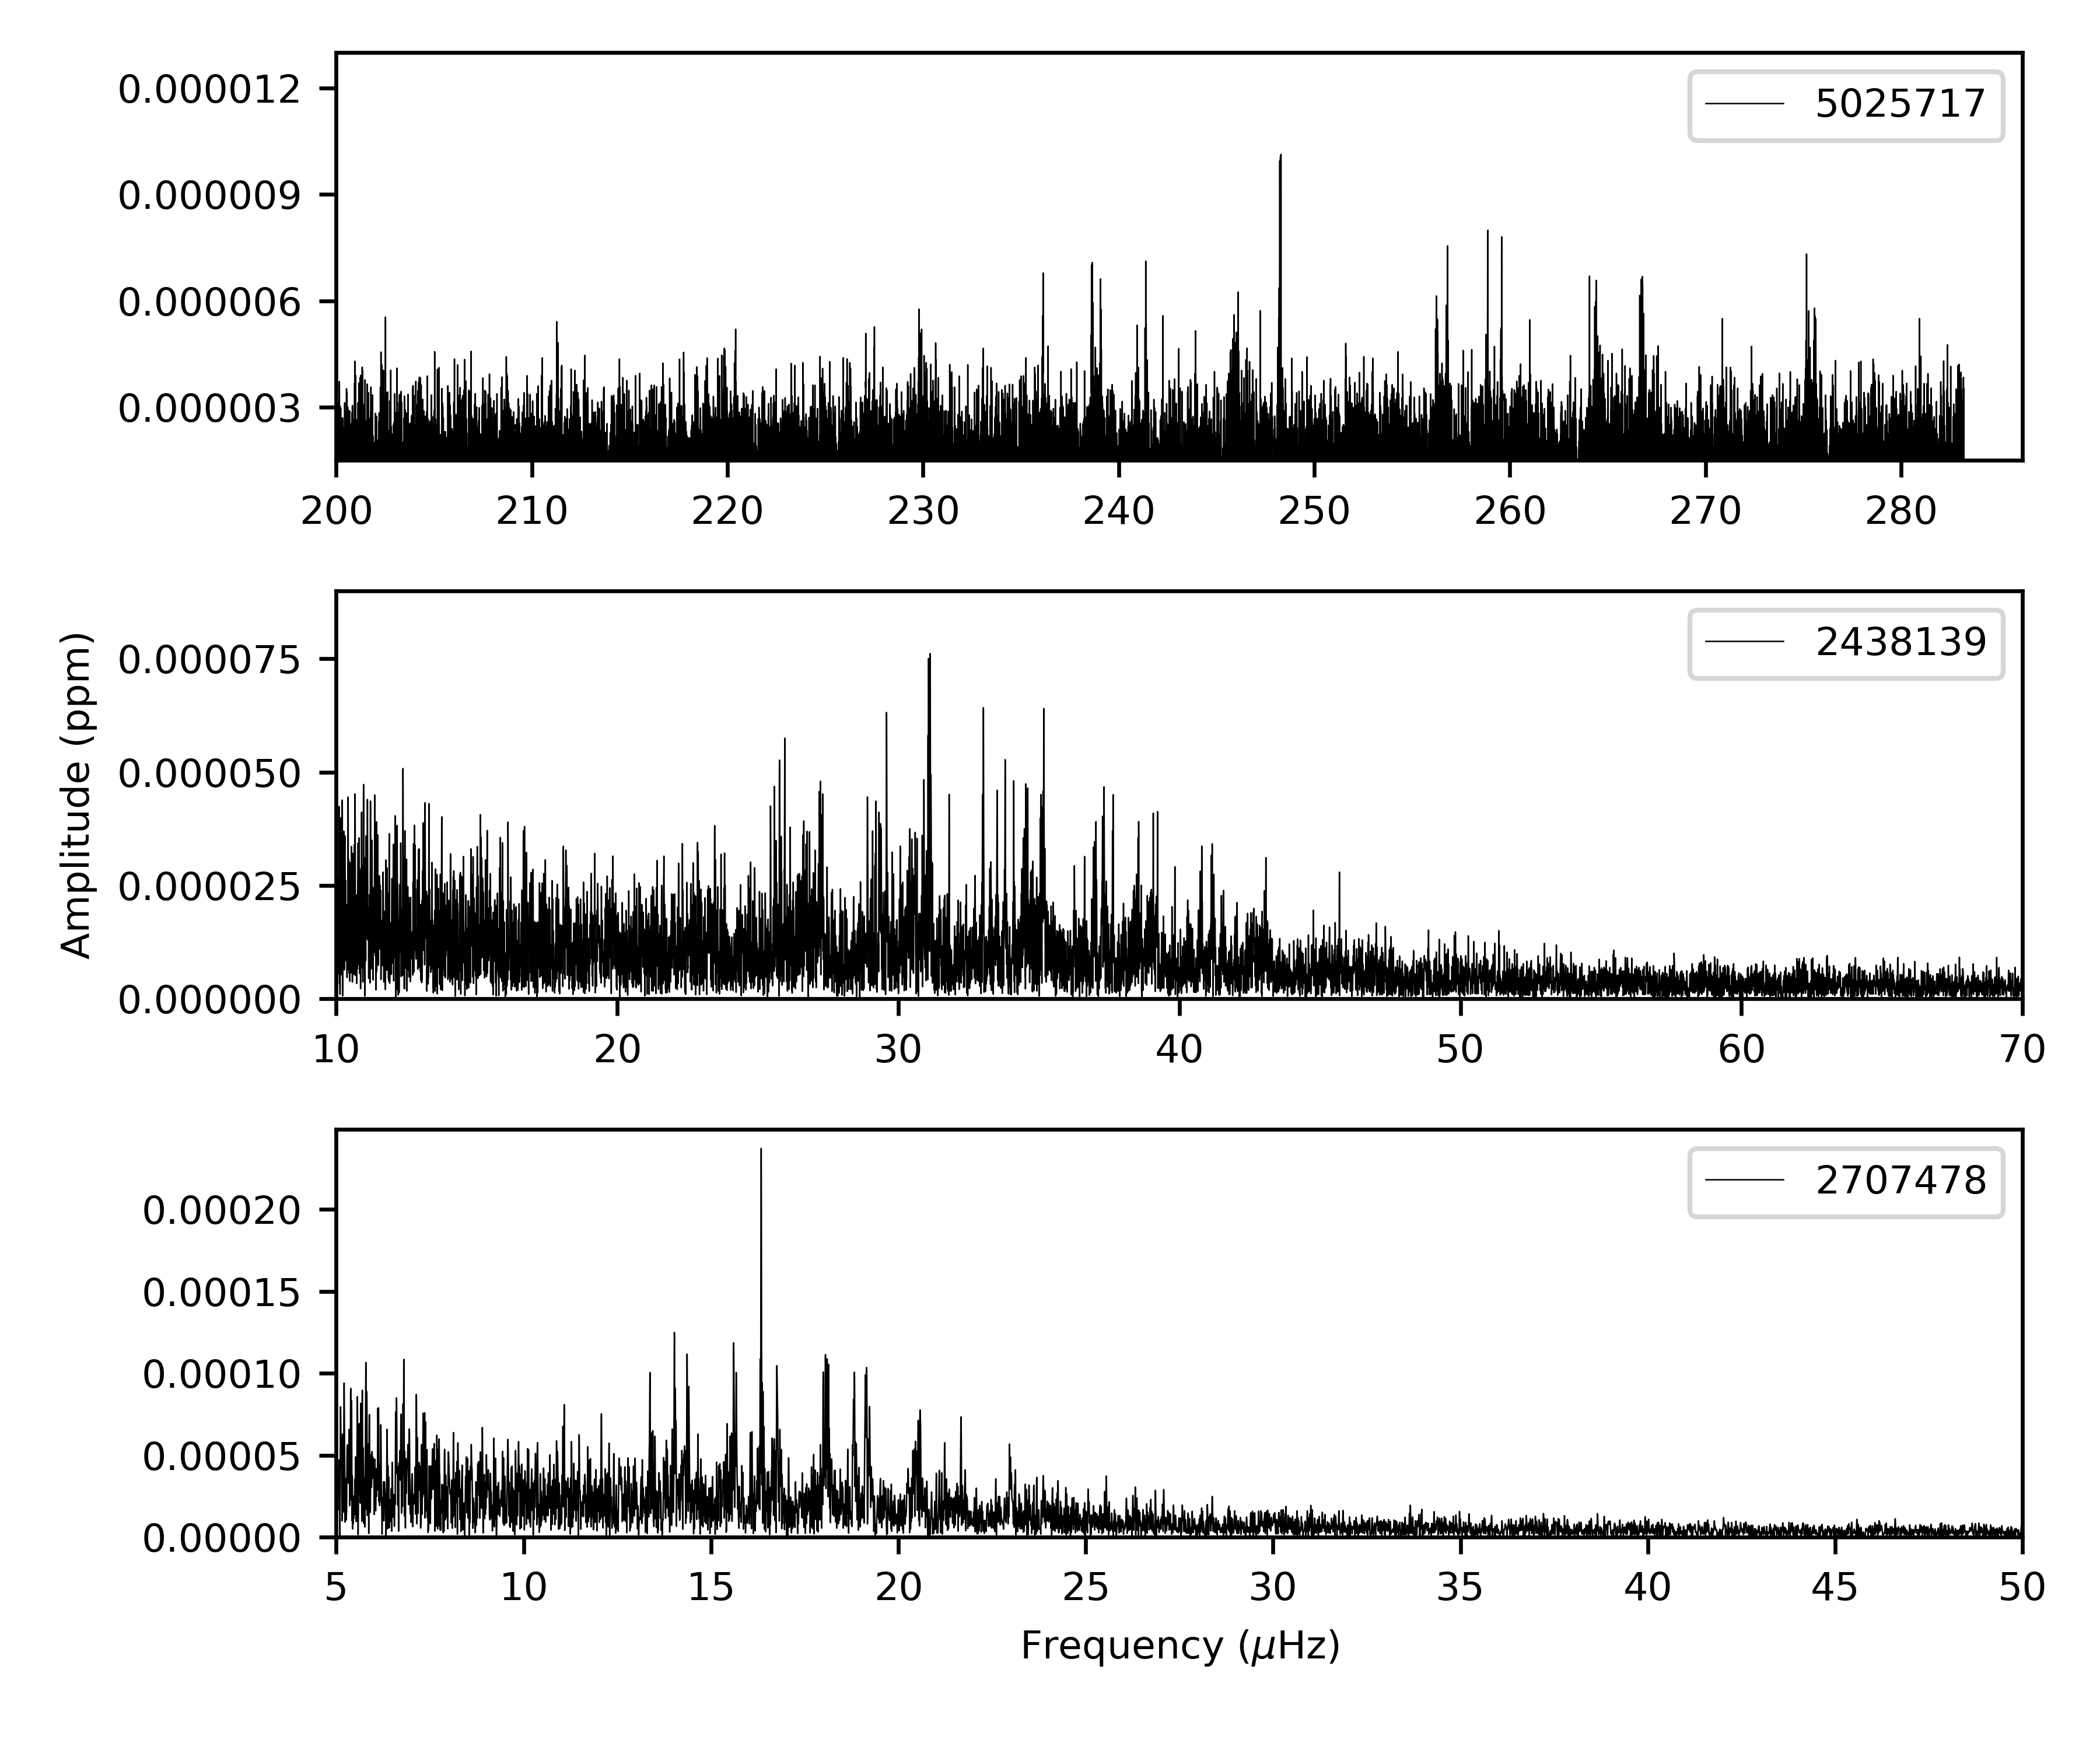
\includegraphics[width=0.95\linewidth]{Chapter5/ebss_ps.png}
    \caption[Amplitude spectra of three potential evolved blue straggler stars]{Amplitude spectra of the three potential evolved blue straggler stars we have identified in NGC\,6791 and NGC\,6819 showing solar-like oscillations.}
    \label{fig:ebss}
\end{figure}


\subsubsection{\numax{} \textendash \dnu{} relation}

\cite{hekker_characteristics_2009} first showed the tight correlation between \dnu{} and \numax{} for red giants using \textsc{CoRoT} data. This relation has since been further investigated \cite[eg.][]{stello_relation_2009, huber_testing_2011}, with \cite{yu_asteroseismology_2018-1} conducting the most detailed investigation to date, using over 16,000 red giants. \cite{ hekker_asteroseismic_2011} first produced this plot for the cluster ensembles of NGC\,6791 and NGC\,6819, including 46 and 42 red giant members, respectively. Figure \ref{fig:nike_6791} presents an updated view of this diagram (top panel) with 150 and 131 red giant members for NGC\,6791 and NGC\,6819, respectively, more than doubling the number of cluster members in each case. The grey points in this figure present the field star sample (Yc) for comparison. 

\cite{yu_asteroseismology_2018-1} showed a modified version of this plot, with \numax{}$^{0.75}$/\dnu{} plotted on the ordinate axis. This new axis removes the diagonal trend and highlighted the trend of increasing mass with increasing ordinate value. This trend enables us to use the ordinate axis as a proxy for stellar mass. We produced similar plots for each cluster (bottom panel), and note that clear isochrones for each cluster are superimposed on the field distribution. The red giants in NGC\,6819 form a horizontal population, and reveal a near constant mass, whilst the red clump and evolved red giant stars appear as an excess within the \numax{} range of $\sim25$\textendash{}$35\,\mu$Hz for NGC\,6791 and $\sim40$\textendash{}$50\,\mu$Hz for NGC\,6819. In both clusters, but particularly in NGC\,6791 this excess lies slightly below a linear fit to the stars outside this \numax{} range. Since the ordinate axis is a proxy for mass, this confirms the clear mass-loss measured by \cite{miglio_asteroseismology_2012} in NGC\,6791, with a more complete sample of the cluster red giants, and hints at a negligible mass-loss within NGC\,6819 red clump stars. In addition, we have provided a comparison to the distribution of field red giants for the first time.

\begin{figure}
    \centering
    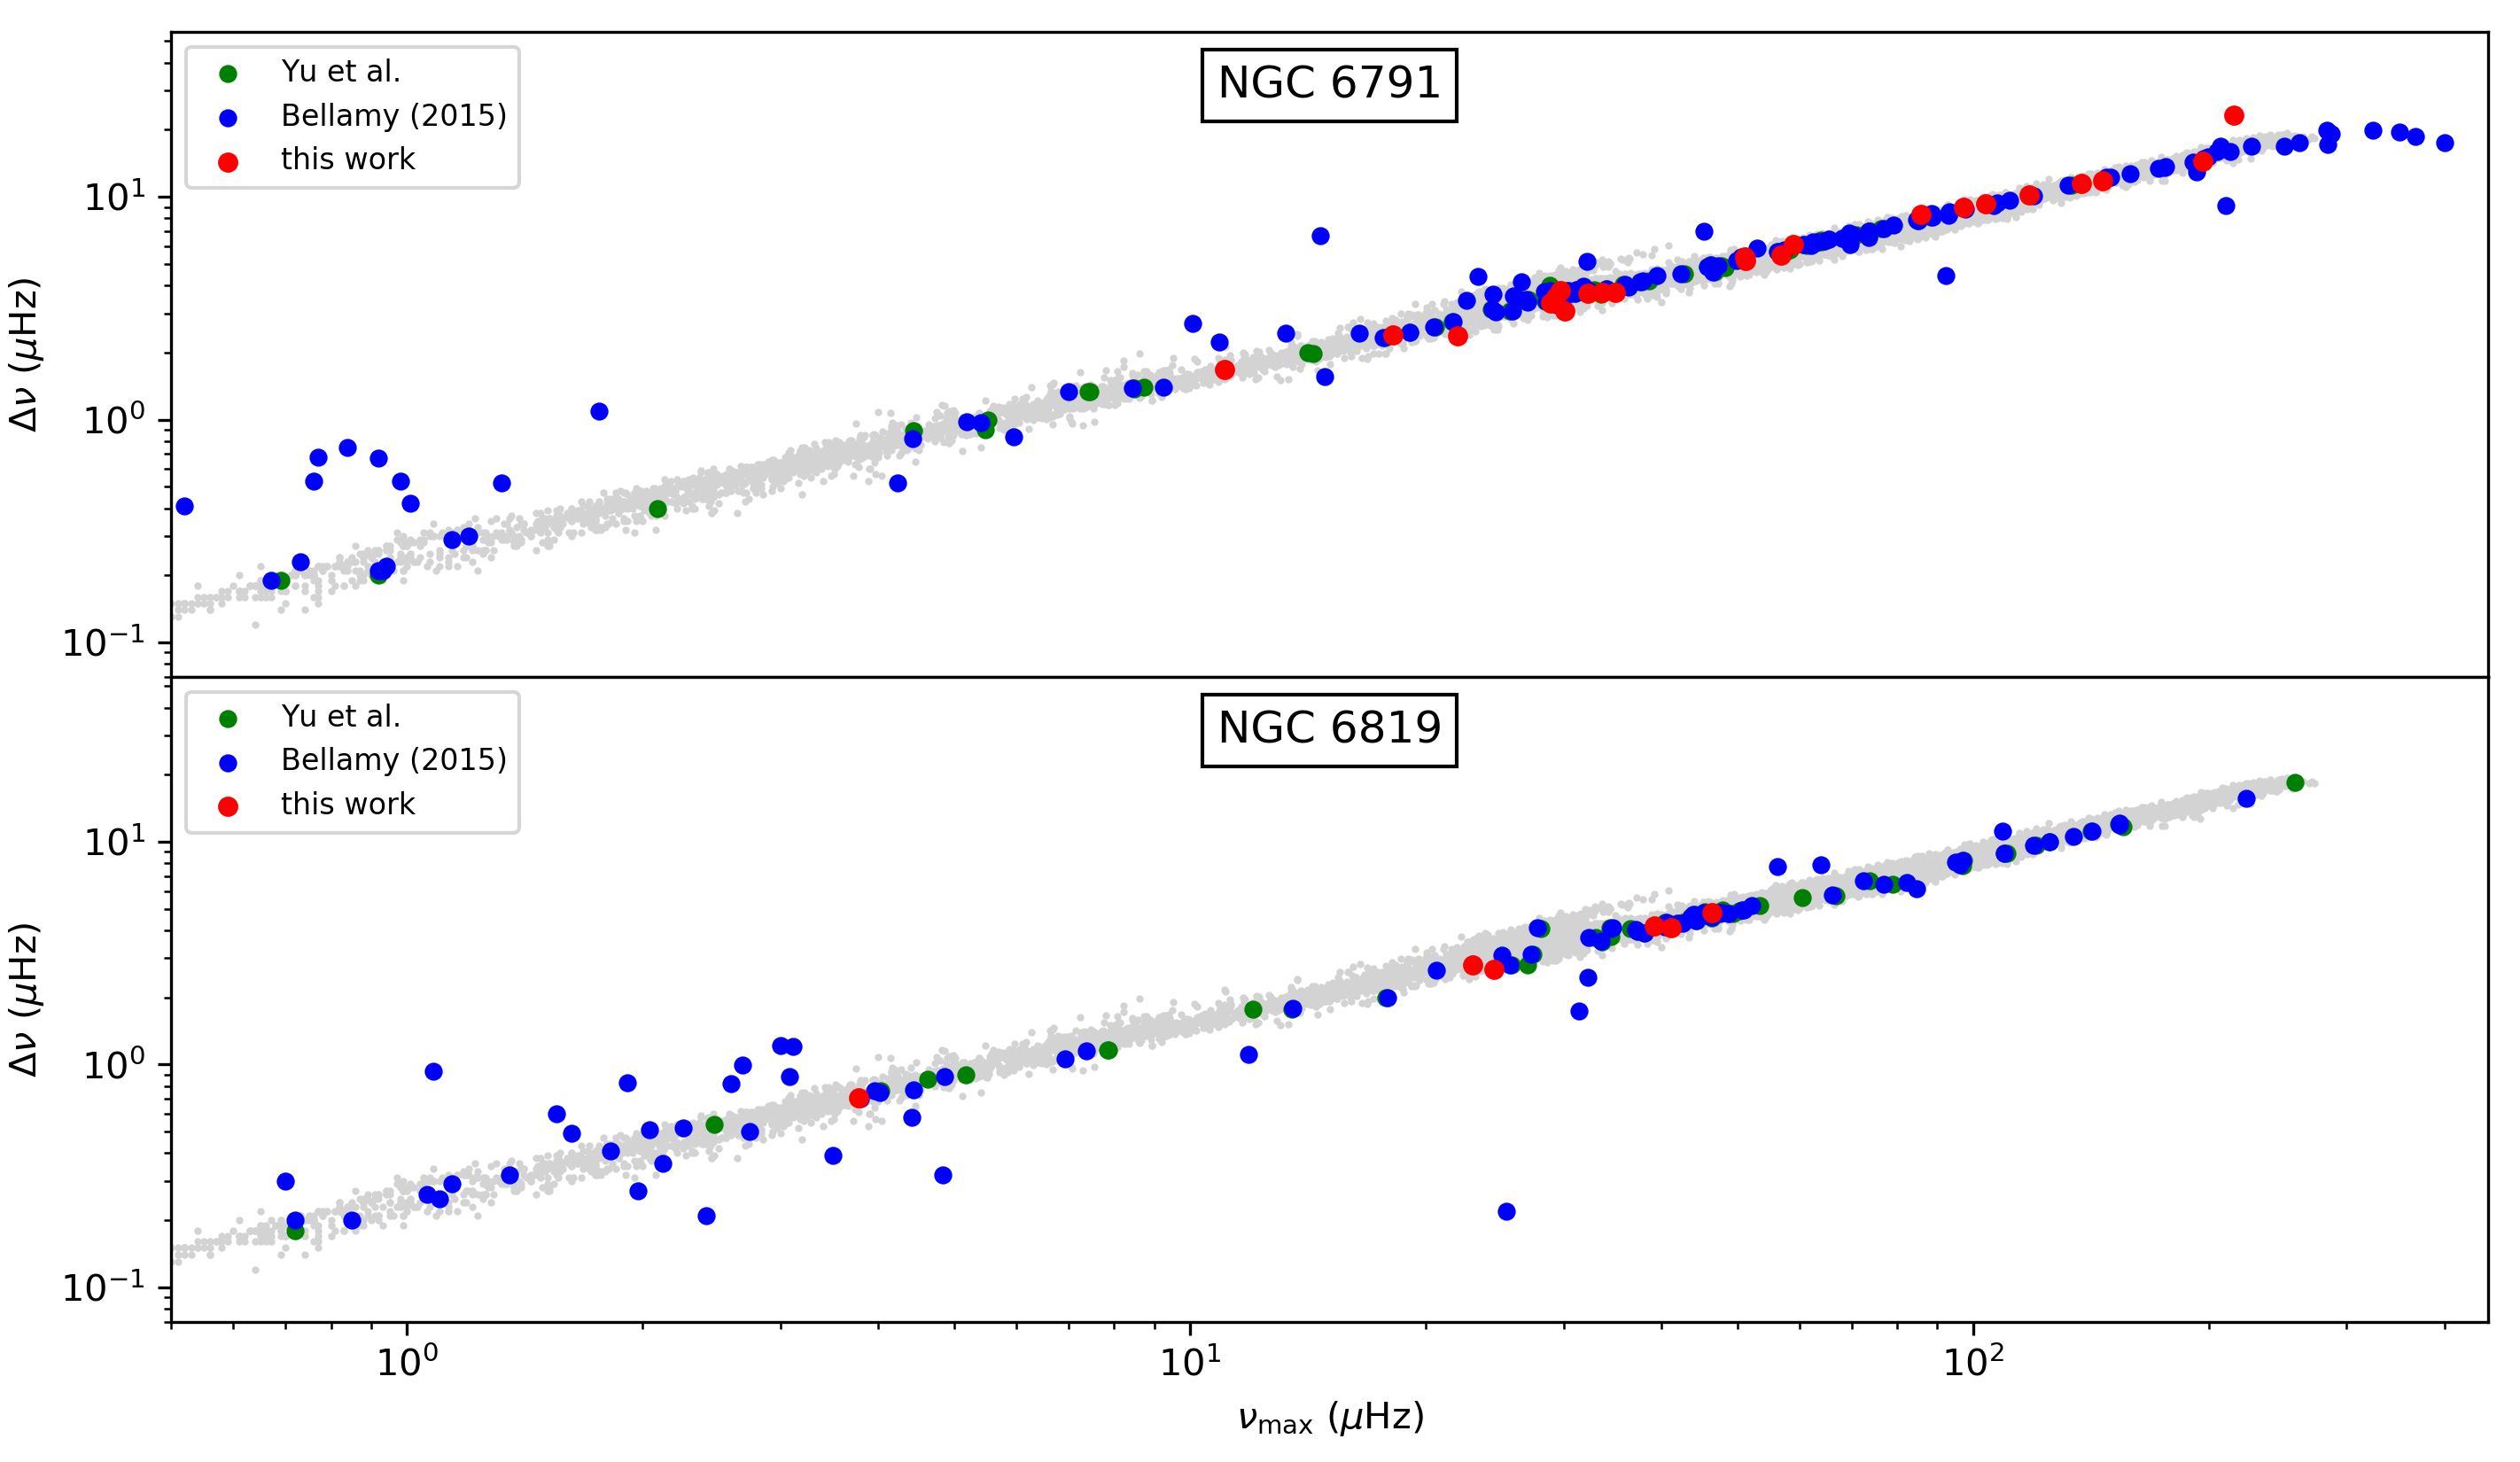
\includegraphics[width=\linewidth]{Chapter5/numax_dnu_both_2.png}
    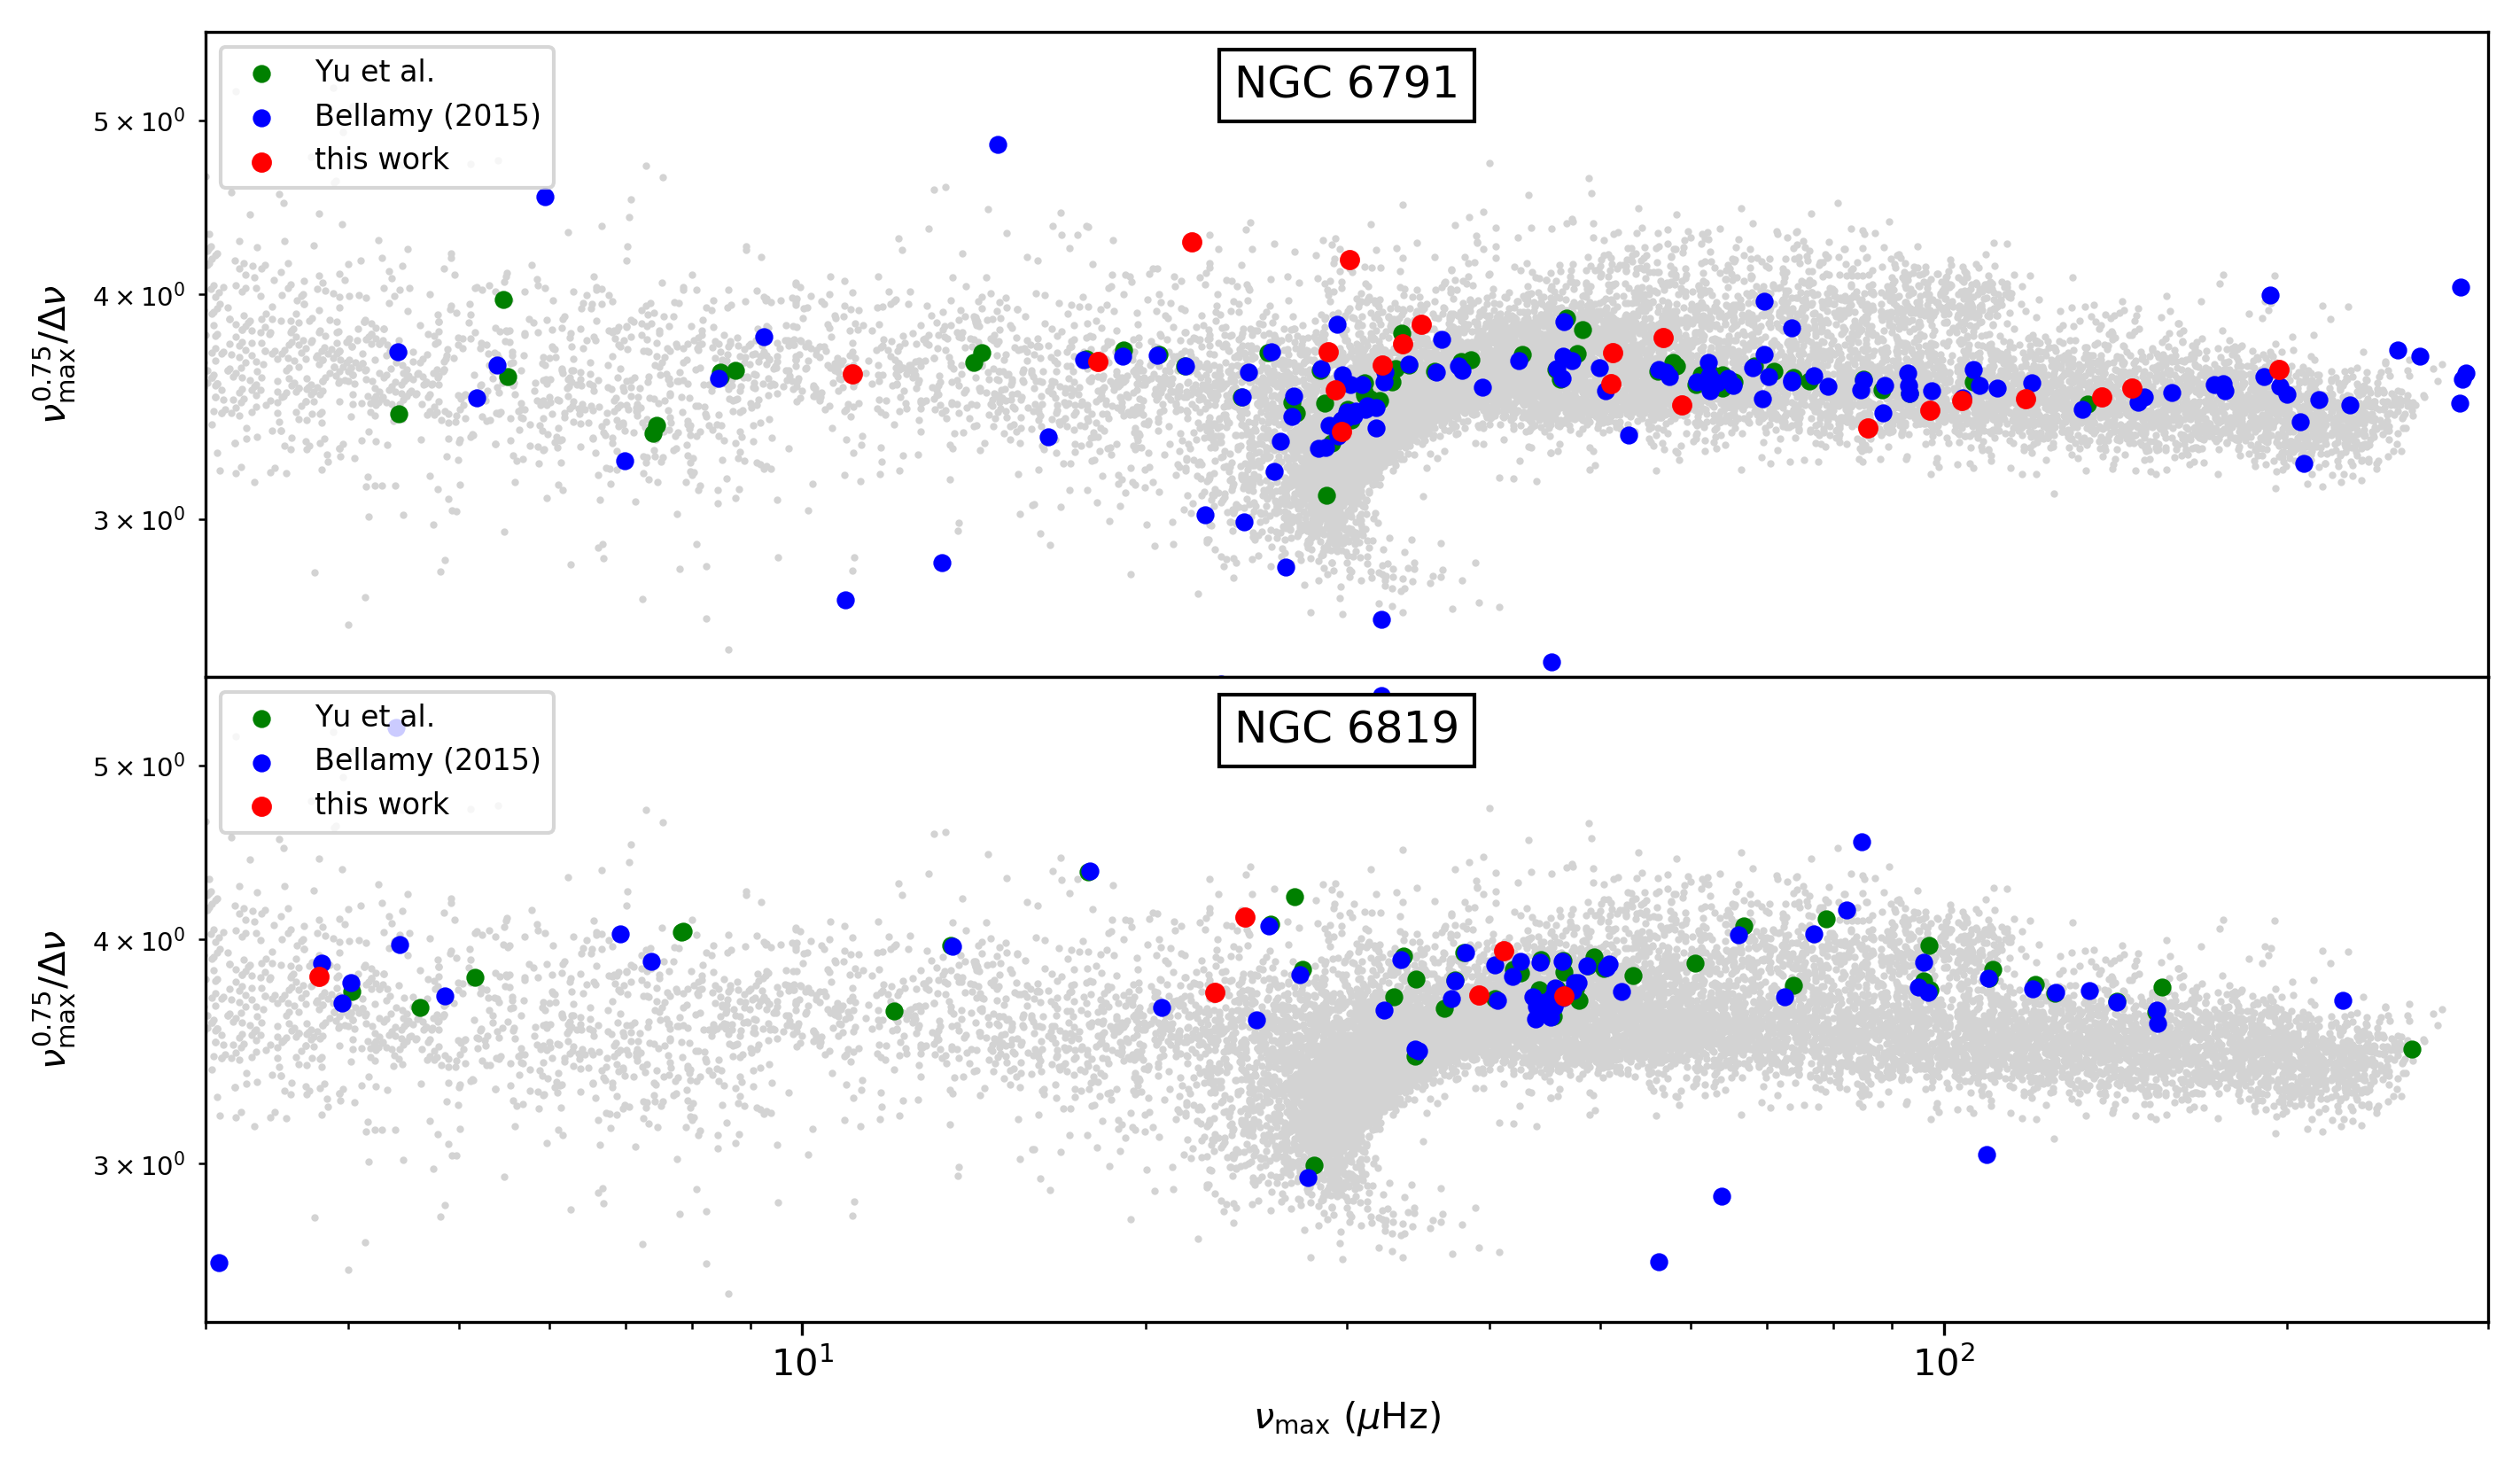
\includegraphics[width=\linewidth]{Chapter5/numax_dnusc_both_2.png}
    \caption[\numax{} \textendash \dnu{} diagram for NGC\,6791 and NGC\, 6819]{\numax{} \textendash \dnu{} diagram for NGC\,6791 (top) and NGC\,6819 (bottom). The ensemble from \cite{yu_asteroseismology_2018-1} (grey) are overlaid with the cluster members (Chapter \ref{chap:membership}) from \cite{yu_asteroseismology_2018-1} and \cite{yu_asteroseismology_2020} (green), \cite{bellamy_using_2015} (blue) and those we have newly extracted values for from this work (red). }
    \label{fig:nike_6791}
\end{figure}

\subsubsection{$\epsilon$ \textendash $\Delta\nu$ Diagram}

\cite{huber_asteroseismology_2010} and \cite{mosser_mixed_2011} showed that \dnu{} is also highly correlated with the phase term, $\epsilon$, for red giants. \cite{corsaro_asteroseismology_2012} plotted this relation for the cluster ensembles and presented fits for:

\begin{equation}
    \epsilon = A + B \mathrm{log}\Delta\nu
\end{equation}

\noindent in agreement with those found by \cite{mosser_universal_2011} for \textsc{CoRoT} red giants and \cite{kallinger_evolutionary_2012} for $\sim$900 \Kepler{} red giants with 600\,days of data. We have recreated this diagram for the complete sample of \Kepler{} red giant field stars, overlaid with our complete ensemble of cluster members in Figure \ref{fig:eps_6791}. Yc did not measure $\epsilon$ values for the cluster red giants so we have constructed the field distribution with values quoted by \cite{hon_deep_2018}, which were reproduced from \cite{stello_suppression_2016}.  This is the first time the ensemble of cluster red giants has been overlaid on the field distribution, and clear isochrones are apparent for each cluster, tracing lines of almost constant mass. The red clump distributions form distinct groups for each cluster, with slightly lower $\epsilon$ values than the red giants with similar \dnu{} values. This is consistent with the cluster isochrones shown by \cite{corsaro_asteroseismology_2012}.

\begin{figure}
    \centering
    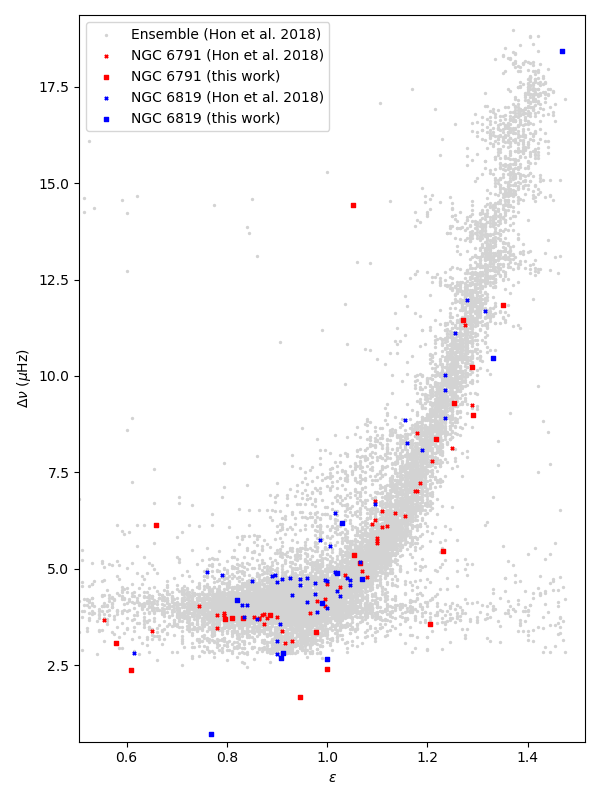
\includegraphics[height=0.5\textheight]{Chapter5/epsilon_combined.png}
    \caption[$\epsilon$ \textendash \dnu{} diagram for NGC\, 6791 and NGC\, 6819 cluster members]{$\epsilon$ \textendash \dnu{} diagram for NGC\,6791 (red) and NGC\,6819 (blue) cluster members with values from \cite{hon_search_2019} (circles) and this work (squares) overlaid on the red giant field distribution}
    \label{fig:eps_6791}
\end{figure}

\section{Conclusions}

In this chapter, we have presented a complete sample of cluster red giants for NGC\,6791 and NGC\,6819, to the limit of red giant oscillation detections. We have re-classified some stars that we found to be likely astrometric members to be non-members based on their photometric variability. This allowed us to produce an improved cluster membership determination compared to our membership in Chapter \ref{chap:membership}. We have also shown clear isochrones exist for each cluster in both the \numax{} - \dnu{} and $\epsilon$ - \dnu{} relations, and have produced updated asteroseismic diagrams for the cluster red giant ensembles, with the field distribution included for the first time for comparison with these isochrones.



% \section{Seismic Membership}

% Following \cite{stello_asteroseismic_2011} and \cite{bellamy_new_2015} we calculated global \numax{} and \dnu{} parameters for each star based on the scaling relations, and assuming the distance modulus, average red giant mass, and metallicity of the clusters shown in \cref{tab:cluster_params}.

% \begin{figure}
%     \centering
%     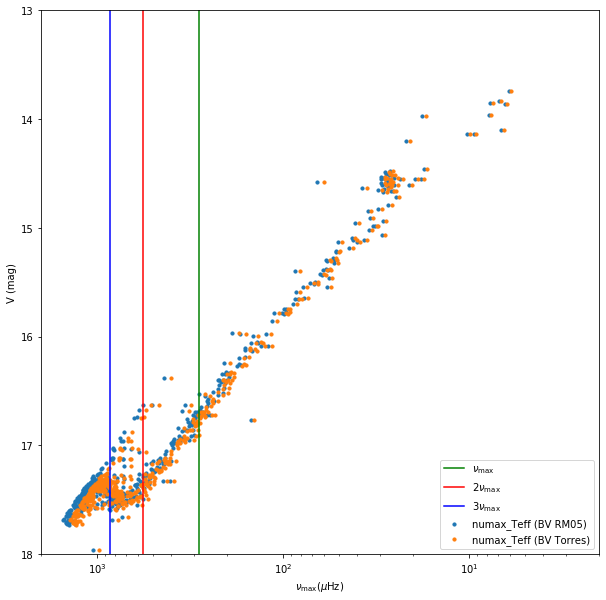
\includegraphics[width=0.48\linewidth]{Chapter5/numax_pred.png}
%     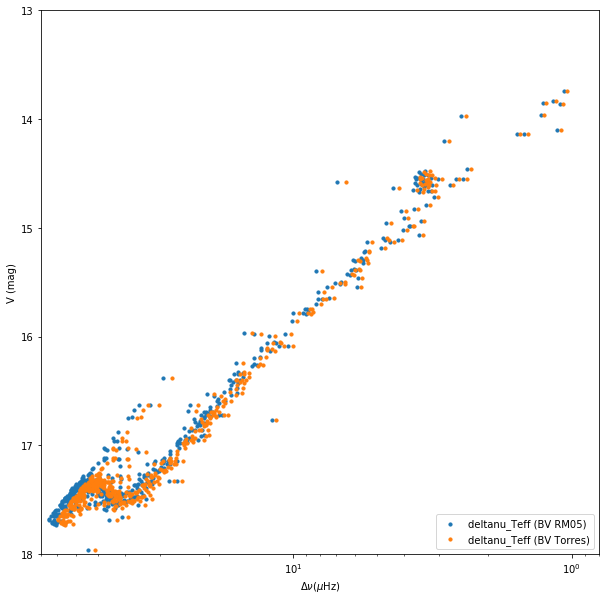
\includegraphics[width=0.48\linewidth]{Chapter5/deltanu_pred.png}
%     \caption{Caption}
%     \label{fig:predicted_seismic}
% \end{figure}

% \begin{table}[h]
%     \centering
%     \begin{tabular}{c|cc|cc}
%             & \multicolumn{2}{c}{{\bf NGC\,6791}} & \multicolumn{2}{c}{{\bf NGC\,6819}}   \\
%         & {\bf Value}   & {\bf Reference}           & {\bf Value}  & {\bf Reference}              \\
%         $m-M_0$     & 13.09   & \cite{wu_asteroseismic_2014}      & 11.747 & \cite{abedigamba_distance_2016}\\
%         RG Mass     & 1.23    & \cite{miglio_asteroseismology_2012}  & 1.61   & \cite{miglio_asteroseismology_2012}\\
%         Metallicity & 0.34    &                     & 0.09   &                        \\
%     \end{tabular}
%     \caption{Global cluster parameters used to calculate the asteroseismic global parameters for each red giant based on the scaling relations.}
%     \label{tab:cluster_params}
% \end{table}

% \begin{figure}
%     \centering
%     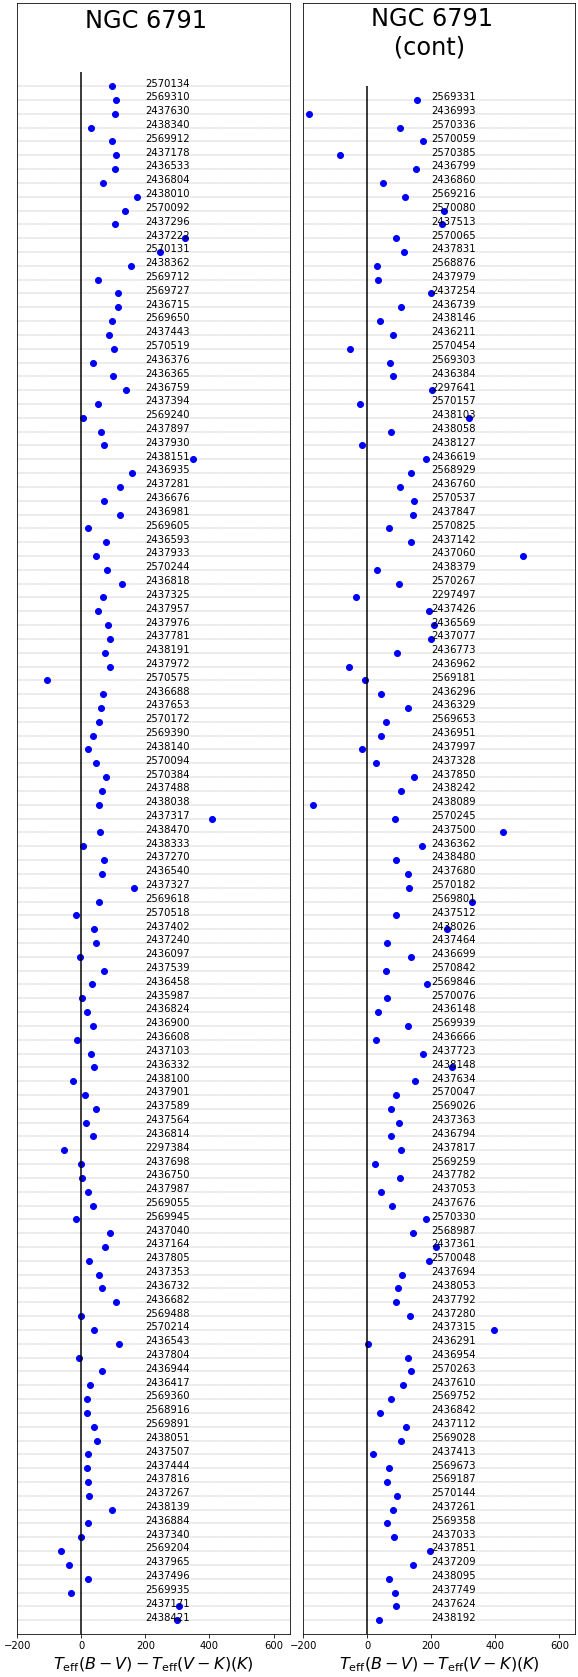
\includegraphics[height=1.75\linewidth]{Chapter5/teff_comp.png}
%     \caption{Caption}
%     \label{fig:teff}
% \end{figure}



%Teff calculation and comparison.


% \section{Asteroseismology}

% \section{Solar-like Oscillators}
% \subsection{Red giants}

% \subsection{Subgiants}

% \section{Eclipsing binaries}

% \section{RR Lyrae oscillators}
% \newpage
% \section{Acknowledgements}

% The author would like to thank Daniel Hey, as well as supervisors Tim Bedding and Dennis Stello for many helpful discussions, direction and suggestions that have enabled this chapter. Daniel Hey developed the echelle routine and provided helpful discussions and debugging suggestions for the initial Pymc3/exoplanet routine that evolved into the one used here to extract numax.
%The author acknowledges the Sydney Informatics Hub and the University of Sydney’s high performance computing cluster, Artemis, for providing the computing resources that have contributed to the results reported herein.